\documentclass [bachelor,german,a4paper,11pt,oneside,webreferences,noglossary,acronym,listofabbrev,indextop,nolistoftables,listoflistings,nolistofalgorithms,noacknowledgements]{INSOthesis}
% change encoding in the document
\inputencoding{utf8} % default
%\inputencoding{latin1} % for windows

\thesistitle{Evaluierung von REST Frameworks für Android}
\thesisshorttitle{Evaluierung von REST Frameworks}
\thesissubtitle{im Kontext des Revex2020 Projekts} % optional
\thesisdate{\today}

% all titles and designations have to be gender-related!
%\thesistype{Diplomarbeit}{Master's Thesis}
%\thesisdegree{Diplom-Ingenieurin}{Diplom-Ingenieurin}
\thesiscurriculum{Software \& Information Engineering}{Software \& Information Engineering} % your study
\thesisauthor{Elisabeth Pilz} % your name
\thesisauthoraddress{Luegstraße 13, 3340 Waidhofen Ybbs} % your address
\thesismatrikelno{1225231} % your registration number

% advisor
%\thesisauthorpreamble {Verfasser}
%\thesisadvisorpreamble {Betreuung}
%\thesisadvisorone {Thomas Grechenig}
\thesisadvisortwo {Dominik Moser}
%\thesisadvisorthree {Vorname Nachname}

% Bibliographie file
\bibliography{bibliography/references}
\hypersetup{
  %colorlinks=false % enable and disable frames arround links
}

%%%%%%%%%%%%%%%%%%%%%%%%%%%%%%%%%%%%%%%%%%%%%
%
% Can be used to add additional informations
%
%%%%%%%%%%%%%%%%%%%%%%%%%%%%%%%%%%%%%%%%%%%%%
% \AfterTitlePages{}
% \AfterDeclaration{}
% \AfterAcknowledgements{}
% \AfterAbstract{}
% \AfterListOfFigures{}
% \AfterListOfTables{}
% \AfterAbbreviations{}
% \AfterBibliography{}
\renewcommand\afterchapternum{\hspace{1em}}
\begin{document}

\maketitle

%%%%%%%%%%%%%%%%%%%%%%%%%%%%%%%%%%%%%%%%%
%%%   CONTENTS    %%%%%%%%%%%%%%%%%%%%%%%
%%%%%%%%%%%%%%%%%%%%%%%%%%%%%%%%%%%%%%%%%


%%%%%%%%%%%%%%%%%%%%%%%%%%%%%%%%%%%%%%%%%%%%%%%%%%%%%%%%%%%%%%%%%%%%%%%%
\chapter{Einleitung}
\label{sec:introduction}
%%%%%%%%%%%%%%%%%%%%%%%%%%%%%%%%%%%%%%%%%%%%%%%%%%%%%%%%%%%%%%%%%%%%%%%%

%=======================================================================
\section{Problemstellung}
%=======================================================================
Einer der größten Trends auf den Business-Markt ist die Mobilisierung der Geschäftswelt, die sich in den verschiedensten Unternehmensstrategien widerspiegelt. Es gibt zahlreiche Innovationen, um unabhängig von Stakeholdern, Zeit, Ort und Geräten auf Daten und Anwendungen zuzugreifen. Ein wesentlicher Innovationsstrang ist dabei die Entwicklung von Business-Apps, um beispielsweise die Arbeitszeiten auf Geschäftsreisen effektiv ausnützen zu können. Dadurch hat die Bedeutung der Informations- und Kommunikationsindustrie in den letzten Jahren in den Unternehmen stetig zugenommen \cite{smartMobileApps1}.
\\\\
Durch die immer stärkere Nachfrage nach mobilen Apps im Arbeitsalltag ist es notwendig, mobile Endgräte in bestehende Geschäftsprozesse der Unternehmen zu integrieren. Dabei soll es vermieden werden, eine komplett neue IT-Infrastruktur unter Beteiligung von mobilen Endgeräten zu schaffen. In vielen Unternehmen wird daher die IT-Anwendungslandschaft an das Paradigma der serviceorientierten Architektur ausgerichtet. Ein wesentlicher Vorteil dabei ist, dass wohl definierte Schnittstellen vorhanden sind und angebotene Dienste flexibel und plattformunabhängig genutzt werden können. Sollen nur mobile Anwendungen in die existierende IT-Anwendungslandschaft eingegliedert werden, bedeutet dies in der serviceorientierten Architektur, das Web Services benötigt werden. In der Praxis werden Web Services entweder mit dem Kommunikationsprotokoll \acrfull{SOAP} oder \acrfull{REST} umgesetzt \cite{smartMobileApps17}.
\\\\
Im Revex2020 Projekt wird das Kommunikationsprotokoll REST verwendet, dadurch ist es nötig ein geeignetes Framework aufseiten der mobilen App zu finden, dass eine vollständige und korrekte Anbindung an den Webservice ermöglicht. Es existieren bereits zahlreiche Frameworks, die eine REST Implementierung unterstützen, diese unterscheiden sich aber stark in der Qualität und im Funktionsumfang. Auch bieten nicht alle diese Frameworks eine Unterstützung für Android an. Daher ist die Auswahl eines geeigneten Frameworks für eine erfolgreiche Implementierung ausschlaggebend. 

%=======================================================================
\section{Motivation}
%=======================================================================

Die Thematik rund um REST-Frameworks für Android ist noch relativ neu, dadurch ist es nicht möglich ohne größere Recherchen ein geeignetes Framework für das Projekt Revex2020 auszuwählen. Es gibt zwar einige Vergleiche von REST Frameworks, wie etwa die Fachstudie von Markus Fischer, Kalman Kepes und Alexander Wassiljew \cite{vergleich13}. In dieser Studie wird allerdings nicht darauf eingegangen, ob die Frameworks eine Implementierung clientseitig mit Android unterstützen, es wird die vermehrt auf die serverseitige Implementierung eingegangen. Die Möglichkeit der clientseitigen Implementierung ist aber eine essenzielle Anforderung, da eine Business-App für Android entwickelt werden soll. 
\\\\
Der immer stärker wachsende Bereich von mobilen Anwendungen macht das zu untersuchende Thema besonders interessant. Herkömmliche Software rückt immer weiter in den Hintergrund, Daten sollen sofort und überall abgerufen werden können. Mobile Endgeräte wie Smartphone und Tablets verändern daher die Geschäftswelt nachhaltig, Führungskräfte und Mitarbeiter erhalten jederzeit Zugang zu Unternehmensinformationen und -prozessen. Die Unternehmen der Zukunft werden daher mobil \cite{smartMobileApps7}.  
\\\\
Revex2020 ist ein Forschungsprojekt zur Revitalisierung von Wasserkraftwerken, das in Kooperation mit dem Institut für Energietechnik und Thermodynamik entwickelt wird \cite{doujak}. Ein Ziel dieses Projektes ist es, Mitarbeitern zukünftig zu ermöglichen, mithilfe von mobilen Endgeräten den Zustand einzelner Kraftwerkskomponenten vor Ort erfassen zu können. Es soll eine Android-App entwickelt werden, die das bereits vorhandene Backend, über das REST-Webservices nutzt um exemplarisch den Anwendungsfall abzubilden.

%=======================================================================
\section{Zielsetzung}
%=======================================================================

Ziel dieser Bachelorarbeit ist die Evaluierung verschiedener REST-Frameworks für Android im Kontext des Revex2020 Projekts, um eine unkomplizierte Anbindung an das bereits vorhandene Backend zu ermöglichen. Dazu werden bestehende REST-Frameworks für Android getestet, indem diese in einem Anwendungsfall eingesetzt werden. Nach der Evaluierung dieser Frameworks soll eine Empfehlung abgegeben werden, welches sich am besten für das Revex2020 Projekt eignet.
\\\\
Die Evaluierung der Frameworks erfolgt anhand von Prototypen, indem die REST-Frameworks verwendet werden. Es wurden im Vorfeld verschiedene Anwendungsfälle definiert (siehe Abbildung \ref{figure:useCase}), indem die einzelnen REST Frameworks integriert werden. Dabei werden in einem Szenario verschiedene Prozesse durchgespielt, wie Kraftwerk erstellen, löschen, bearbeiten und anzeigen. Als Vorlage dazu wurde die bestehende Web-Applikation des Projektes verwendet.
\\\\

\begin{minipage}{\textwidth} 
	\centering	
	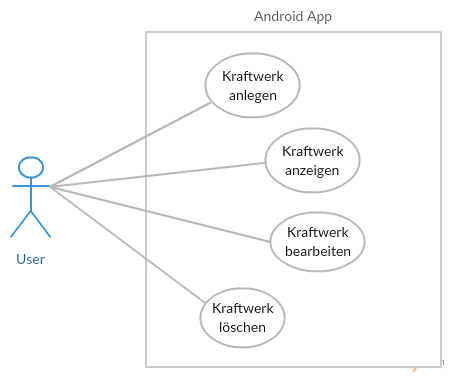
\includegraphics[width=0.65\textwidth]{figures/kraftwerke_use_case.png}
	\captionof{figure}{Use-Case-Diagramm}
	\label{figure:useCase}
	\vspace{2ex}
\end{minipage}

%=======================================================================
\section{Methodik}
\label{sec:methodik}
%=======================================================================
Die Qualität der einzelnen Frameworks soll anhand folgender Kriterien verglichen werden, welche an dem Kriterienkatalog der Fachstudie "Vergleich von Frameworks zur Implementierung von REST-basierten Anwendungen" \cite{vergleich13} angelehnt sind. Dieser Kriterienkatalog beschäftigt sich mit den Eigenschaften für die Evaluierung von REST Frameworks, vor allem auf serverseitiger Sicht. Der Kriterienkatalog wurde deshalb gekürzt bzw. einzelne Punkte zusammengefasst und abgeändert, um eine Evaluierung im Kontext des Projektes Revex2020 durchführen zu können. 
\\\\
Das Hauptaugenmerk der Evaluierung liegt auf der Clientseite, da die entwickelte App eine Client Applikation darstellt. Deswegen wurden spezifische Kriterien der Fachstudie zu einer REST Server Applikation gestrichen. Beispielsweise wurde der gesamte Kriterienblock über Ressourcentypen \cite{ressourcen:rest} weggelassen, da es für die clientseitige Verarbeitung irrelevant ist, welche Ressourcentypen serverseitig implementiert werden können. 
\\\\
\textbf{Entwicklungskultur rund um die Frameworks:}
\begin{itemize}
	\item Unter welcher Lizenz steht das Projekt zur Verfügung?
	\item Existiert eine aktive Community?
	\item Ist eine Dokumentation des Codes vorhanden? (Schnittstellenbeschreibung, JavaDoc)	
	\item Gibt es Hilfestellung für Entwicklung? (Tutorial, Codebeispiele)
\end{itemize}

\textbf{Implementierung der REST-Frameworks:}
\begin{itemize}
	\item Wie aufwendig ist es das Framework ins Projekt einzubinden? 
	\item Welche HTTP-Methoden werden unterstützt? (GET, POST, PUT, DELETE etc.)
	\item Gibt es Möglichkeiten den HTTP-Header zu verändern oder zu erweitern?
	\item Welche Medientypen werden unterstützt? (JSON, HTML, XML etc.)
	\item Kann die URL zum Abfragen von Resourcen dynamisch verändert werden? (z.B. über Parameter steuern)
	\item Gibt es eine Möglichkeit für asynchronen Nachrichtenaustausch?
	\item Wird das HATEOAS-Konzept* unterstützt?
	\item Wird ein Error-Handling unterstützt?	
\end{itemize}

\textbf{Performance und benötige Speicherplatz der Frameworks:}
\begin{itemize}
	\item Wie stark wird die CPU belastet?  
	\item Wie viel RAM wird benötigt? 
	\item Wie schnell erfolgt die Abwicklung einzelner Requests (GET, POST)?
	\item Wie groß ist die erzeugte .apk-Datei?	
\end{itemize}
\newpage
\textbf{Erweiterte Technische Fähigkeiten der Frameworks:}
\begin{itemize}
	\item Wie wird Sicherheit gehandhabt?  (Authentifizierung)
	\item Werden andere Protokolle fernab von HTTP unterstützt?	
	\item Unterstützt das Framework die Entwicklung von Server Applikationen?
	\item Bietet das Framework zusätzliche Dienst fernab der REST-Kommunikation an?
	\item Wird transaktionales Verhalten vom Framework unterstützt? (ACID**-Eigenschaften)\\
\end{itemize}

* Das \textbf{HATEOAS}-Konzept wird in Kapitel \ref{sec:rest} genauer beschrieben.
\\\\
** \textbf{ACID} seht für Atomicity, Consistency, Isolation und Durability. Dieses Konzept beschreibt, dass alle Daten die während einer Transaktion verwendet werden, gesperrt sind und sich nicht ändern dürfen, so lange bis die Transaktion Commited wird oder ein Rollback durchgeführt wird. Das Einhalten dieser Eigenschaften ist wichtig, da die Kommunikation zu Servern über zustandslose REST-Schnittstellen abgewickelt wird. Durch die Zustandslosigkeit der Anfragen kann es bei Fehlern schnell zu einer Dateninkonsistenz auf dem Server kommen \cite{braun:Transaktionen}.

%%%%%%%%%%%%%%%%%%%%%%%%%%%%%%%%%%%%%%%%%%%%%%%%%%%%%%%%%%%%%%%%%%%%%%%%
\chapter{State of the Art}
\label{sec:stateOfTheArt}
%%%%%%%%%%%%%%%%%%%%%%%%%%%%%%%%%%%%%%%%%%%%%%%%%%%%%%%%%%%%%%%%%%%%%%%%

Um Rest Frameworks für die Evaluierung zu finden, wurde eine Technologierecherche durchgeführt. Dabei konnten folgende Projekte gefunden werden, welche eine REST-Anbindung für Android unterstützen:
\begin{itemize}
	\item Resty (\href{http://beders.github.io/Resty/Resty/Overview.html}{http://beders.github.io/Resty/Resty/Overview.html})
	\item Retrofit (\href{http://square.github.io/retrofit/}{http://square.github.io/retrofit/})
	\item RESTlet (\href{http://restlet.com/}{http://restlet.com/})
	\item Spring for Android (\href{http://projects.spring.io/spring-android/}{http://projects.spring.io/spring-android/})
	\item CRest (\href{http://crest.codegist.org/index.html}{http://crest.codegist.org/index.html})
	\item RESTeasy Mobile (\href{http://resteasy.jboss.org/}{http://resteasy.jboss.org/})
	\item RESTDroid (\href{http://pcreations.fr/me/restdroid-resource-oriented-rest-client-for-android}{http://pcreations.fr/me/restdroid-resource-oriented-rest-client-for-android})
	\item Jersey (\href{https://jersey.java.net/}{https://jersey.java.net/})
\end{itemize}

Es würde den Rahmen der Bachelorarbeit überschreiten, all diese gefundenen REST Frameworks zu evaluieren. Es wurde daher einer Vorstudie gemacht, aufgrund derer die Drei populärsten und den Anforderungen adäquatesten Frameworks ausgewählt wurden.
\\\\
Die Popularität eines Frameworks gibt eine gewisse Auskunft über die Qualität, da für diese Frameworks oft besserer Support in Form von Dokumentation zur Verfügung steht. Eine Studie von Chris Parnin\cite{parnin2012crowd} beschäftigen sich damit, wie "'Crowd documentation"' beispielsweise auf Question and Answer (Q\&A) Webseiten, die Hilfestellung zu verschiedenen Frameworks beeinflusst. Verwenden viele Entwickler ein Framework, sind dadurch mehr Fragen auf Q\&A Webseiten vorhanden und dadurch können mögliche Fragen besser beantwortet werden. Durch eine Erhebung der Anzahl von Fragen auf Stack Overflow\footnote{\href{http://stackoverflow.com/}{http://stackoverflow.com/}} und der Stars auf GitHub\footnote{\href{https://github.com/}{https://github.com/}} wurden Rückschlüsse auf die Popularität der einzelnen Frameworks gezogen.  
\\\\
In dem Artikel "'How to identify a strong open source project"\cite{balter:strongOS} werden verschiedene Indikatoren erhoben, welche Rückschlüsse auf eine solide und gute Entwicklung eines Frameworks geben. Deswegen wurden zusätzlich noch verschiedene Aktivitäten auf GitHub verglichen, wie Datum des letzten Commits oder Anzahl der Commits.

\begin{minipage}{\textwidth} 
	\centering	
	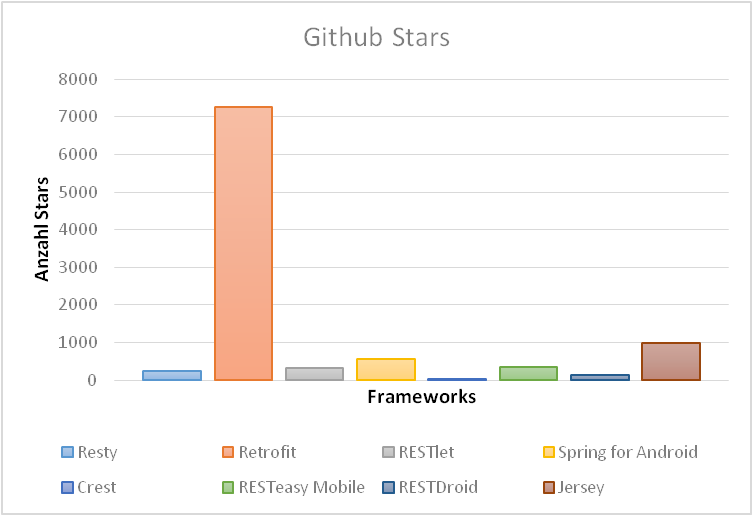
\includegraphics[width=0.65\textwidth]{figures/github_stars.png}
	\captionof{figure}{Github Stars, abgerufen am 25.09.2015}
	\label{figure:githubStars}
	\vspace{2ex}
\end{minipage}

\begin{minipage}{\textwidth} 
	\centering	
	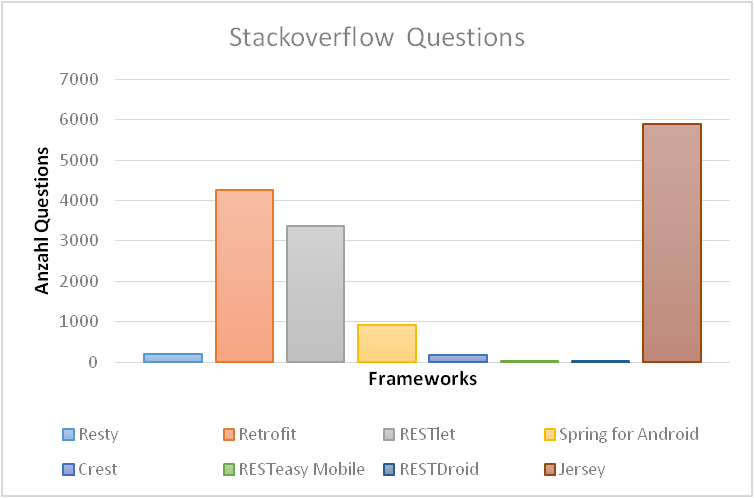
\includegraphics[width=0.65\textwidth]{figures/stackoverflow_questions.png}
	\captionof{figure}{Stackoverflow Questions, abgerufen am 24.09.2015}	
	\label{figure:stackoverflowQuestions}
	\vspace{2ex}
\end{minipage}

\begin{minipage}{\textwidth} 
	\centering	
	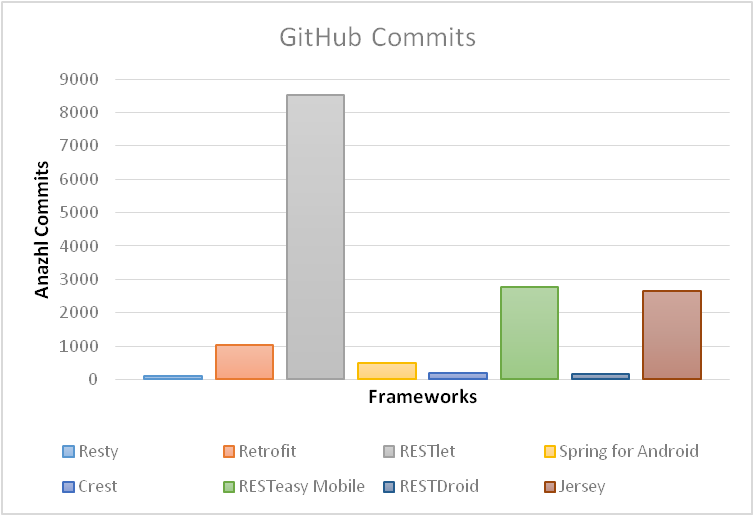
\includegraphics[width=0.65\textwidth]{figures/github_commits.png}
	\captionof{figure}{Github Commits, abgerufen am 25.09.2015}	
	\label{figure:githubCommits}
	\vspace{2ex}
\end{minipage}

\begin{minipage}{\textwidth} 
	\centering	
	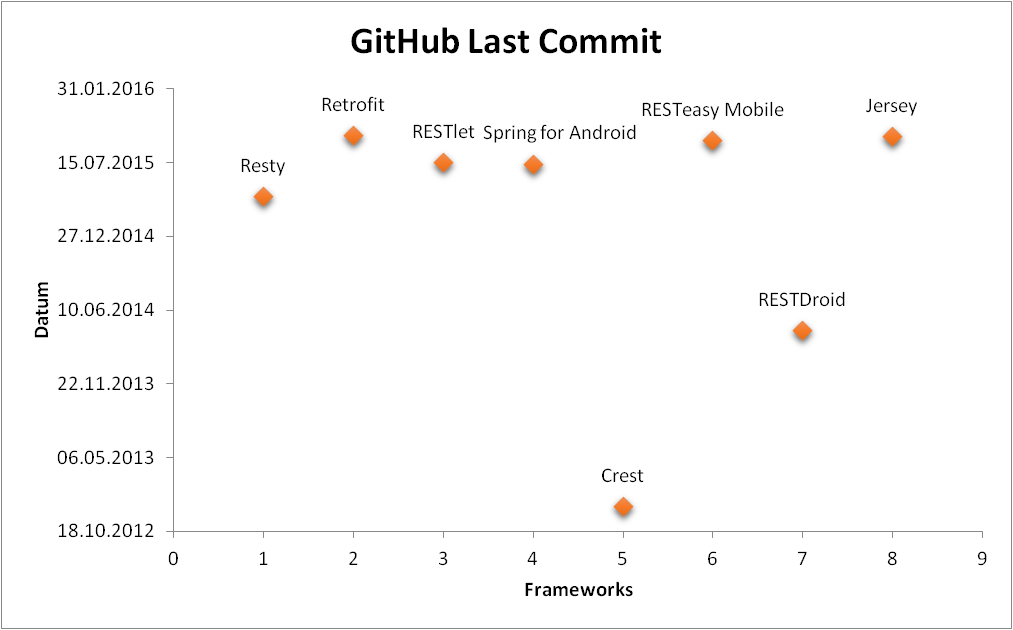
\includegraphics[width=0.65\textwidth]{figures/github_lastCommit.png}
	\captionof{figure}{GitHub Last Commit, abgerufen am 28.09.2015}	
	\label{figure:githubLastCommit}
	\vspace{5ex}
\end{minipage}

Aufgrund der Vorstudie werden folgende REST-Frameworks evaluiert und miteinander verglichen:

\begin{itemize}
	\item Retrofit 
	\item Jersey
	\item Spring for Android
\end{itemize}
%%%%%%%%%%%%%%%%%%%%%%%%%%%%%%%%%%%%%%%%%%%%%%%%%%%%%%%%%%%%%%%%%%%%%%%%
\chapter{Android}
\label{sec:android}
%%%%%%%%%%%%%%%%%%%%%%%%%%%%%%%%%%%%%%%%%%%%%%%%%%%%%%%%%%%%%%%%%%%%%%%%

%=======================================================================
\section{Überblick}
%=======================================================================
Android ist ein Betriebssystems, welches primär für Smartphones und Tablets konzeptioniert ist. Das Betriebssystem basiert auf einen Linux Kernel und wird von der Open Handset Alliance (gegründert von Google) entwickelt \cite{overviewAndroid:singh}. Android ist eine freie Software und das am schnellsten wachsende mobile Betriebssystem. Der Marktanteil von Android liegt seit 2014 bei über 80\% und soll sich auch in den darauffolgenden Jahren bei dieser Prozentzahl halten, wie in der Abbildung \ref{figure:marketshare} zu sehen ist. \\
 
\begin{minipage}{\textwidth} 
	\centering	
	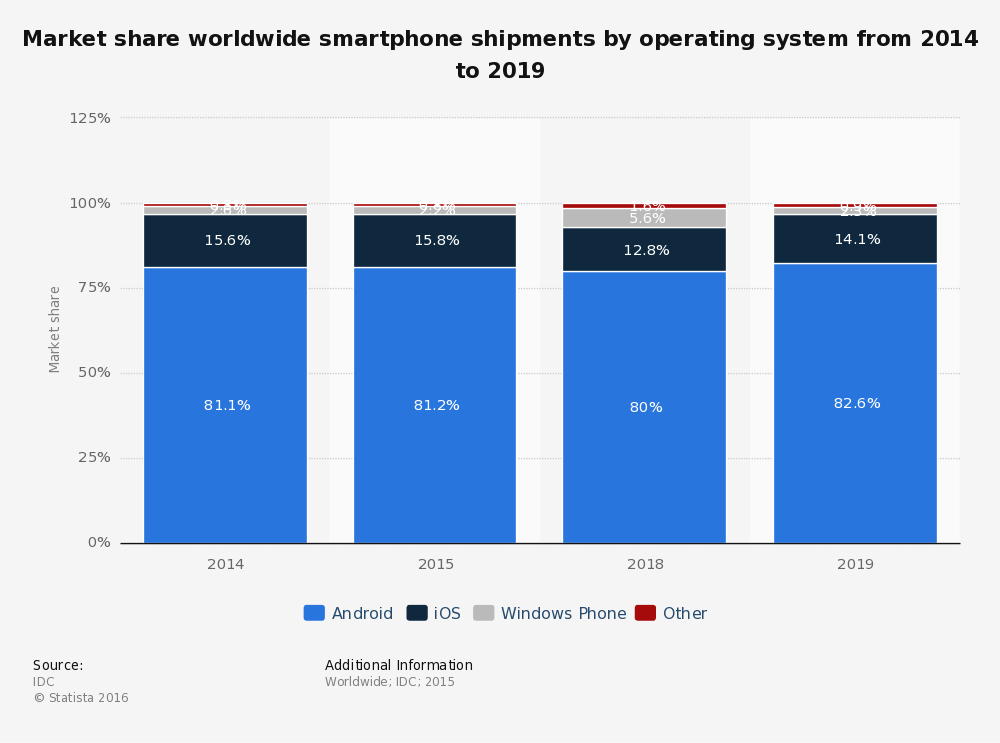
\includegraphics[width=0.65\textwidth]{figures/smartphone-os-market-share.png}
	\captionof{figure}{Marktanteil von mobilen Betriebssystemen \cite{statsticMobileOS}}
	\label{figure:marketshare}
	\vspace{2ex}
\end{minipage}

Durch die quelloffene Struktur des Betriebssystems ist Android bei vielen Konsumenten und Entwicklern sehr beliebt, wodurch viele Unternehmen ihre mobilen Applikationen auf dieses Betriebssystem ausrichten. Gemäß einer Vorhersage von IDC, wird Android zwar eine gewisse Prozentzahl an das Windows Phone Betriebssystem verlieren, aber weiterhin der Marktführer bleiben \cite{statsticMobileOS}. Auf Grund dessen wurde die Evaluierung der REST Frameworks auf Android ausgerichtet, um auch in den folgenden Jahren einen hohen Nutzerkreis erreichen zu können.

%=======================================================================
\section{Architektur}
%=======================================================================
Das Android Betriebssystem ist ein Stack von Software Komponenten, welche typischerweise in vier Bereiche gegliedert werden (vgl. \ref{figure:androidArchitekture}). Diese Bereiche sind der Linux Kernel, die Native Bibliotheken, die Laufzeitumgebung, das Application-Framework und die Applikationen selbst \cite{androidTutorialOS}. \\

\begin{minipage}{\textwidth} 
	\centering	
	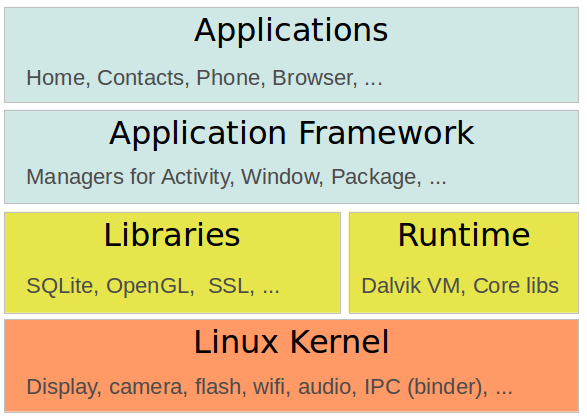
\includegraphics[width=0.65\textwidth]{figures/android_stack.png}
	\captionof{figure}{Android Architektur \cite{androidTutorialOS}}
	\label{figure:androidArchitekture}
	\vspace{2ex}
\end{minipage}

Beschreibung der Software Komponenten der Android Architektur \cite{overviewAndroid:singh}, \cite{androidTutorialOS}: 
\begin{itemize}
	\item \textbf{Applikationen}\\
	Die Applikationen stellen die oberste Schicht der Android Architektur dar. Einige Applikationen sind bereits auf jedem Smartphone vorinstalliert, wie beispielsweise ein SMS Client,  ein Browser oder ein Kontaktmanager. Software Entwickler können ihre eigenen Applikationen schreiben und diese auf dem Smartphone installieren.\\
	Die zu entwickelnde App, sowie die zu evaluierenden REST-Frameworks befinden sich auf dieser Schicht - das REST-Framework und die Beispielimplementierung werden gemeinsam in eine .apk-Datei zusammengefasst.
	\item \textbf{Application-Framework}\\
    In der Application-Framework-Schicht befinden sich zahlreiche Java-Bibliotheken und Dienste, auf welche Software Entwickler bei der Applikationserstellung Zugriff habe. Wichtige Dienste sind dabei der Activity Manager, der Resource Manager oder der Content Manager.
	\item \textbf{Native Bibliotheken}\\
	Die Nativen Bibliotheken stellen zahlreiche Funktionen für die Application-Framework-Schicht zur Verfügung, wie Grafik-Rendering oder Web-Browsing. Alle diese Bibliotheken sind in C oder C++ geschrieben und werden durch Java Interfaces aufgerufen, bei der Entwicklung von Applikationen.
	\item \textbf{Runtime}\\
	Die Laufzeitumgebung besteht aus der Dalvik \acrfull{VM} und den Java Kernbibliotheken. Die Dalvik VM ist eine Java Virtual Machine, welche speziell für Android entwickelt und optimiert wurde.  Durch die  Dalvik VM kann jede Applikation in einem eigenen Prozess ausgeführt werden, mit einer eigenen Instanz der Dalvik VM. \\
	Durch die Java Kernbibliotheken in der Laufzeitumgebung können Software Entwickler Android Applikationen mithilfe der Programmiersprache Java entwickeln.   
	\item \textbf{Linux Kernel}\\
	Der Linux Kernel stellt die unterste Schicht der Android Architektur dar, welcher leicht von Google abgeändert wurde. Der Kernel ist dabei die Schnittstelle zur Geräte Hardware (Kamera, Display etc.) und ist gleichzeitig für die Speicher- und Prozessverwaltung verantwortlich.
\end{itemize}
	
%=======================================================================
\section{Cross Compiling}
%=======================================================================	
Um eine Applikation auf Android ausführen zu können, muss eine .apk-Datei erstellt werden. Dazu wird als erstes eine .java-Datei vom Entwickler erstellt, welche den Quellcode der Applikation enthält. Danach wird mit einem Java-Compiler der Bytecode in Form von .class-Dateien erstellt. Dieser Bytecode wird mit dem dx-Tool aus dem Android SDK in eine .dex-Datei (Dalvik Executable) umgewandelt. Den Bytecode welche die Dalvik VM ausführt ist daher kein Java-Bytecode mehr, sondern Dalvik-Bytecode. Dieser Vorgang wird auch als Cross Compiling bezeichnet. Des weiteren werden mehrere .class-Dateien in eine .dex-Datei zusammengefasst um Speicherplatz zu sparen. Die .dex-Datein werden zusammen mit einem Manifest in eine .apk-Datei verpackt. Diese .apk-Datei wird dann auf das Smartphone übertragen und installiert, wodurch die App ausgeführt werden kann \cite{unterschied:dirscherl}.	

%=======================================================================
\section{Android und Java}
%=======================================================================	
Die meisten Android Applikationen werden in Java geschrieben und haben als Grundlage die Java 6 \acrfull{SE}. Einige Java 7 Funktionalitäten werden ab der Android Versionen 4.4 (KitKat) unterstützt, davor muss darauf geachtet werden, dass keine spezifischen Funktionen von Java 7 verwendet werden \cite{android:burnette}. Dabei unterstützt die Android Java \acrfull{API} einen Großteil der packages welche in der Java SE Bibliothek vorhanden sind. Einige packages wurden aber weggelassen, da sie auf einer mobilen Plattform keinen Sinn machen \cite{implemenationSDK}, wie etwa das Drucken (javax.print). Jedoch wurden zusätzlich einige Drittanbieter Bibliotheken hinzugefügt, um Entwicklern die Arbeit zu erleichtern, beispielsweise die Apache HttpComponents Bibliothek (org.apache.commons.httpclient) \cite{android:libs}. 
\\\\	
Dadurch das Android nicht alle Java SE Funktionen der neuesten Version unterstützt, musste bei der Auswahl der Frameworks darauf geachtet werden, dass diese Java 6 kompatibel sind und keine ausgeklammerten packages verwenden.	

%=======================================================================
\section{Android Versionen}
%=======================================================================
Android veröffentlicht in regelmäßigen Abständen neue Versionen, wie man an den zahlreichen Versionsnummern erkennen kann. Es sind vor allem jene Android-Versionsnummer wichtig, bei denen sich das API-Level ändert. Denn das API-Level bestimmt, welches Geräte eine App ausführen kann und welches nicht. Normalerweise soll eine App von möglichst vielen Geräten ausgeführt werden können. Deswegen sollte ein API-Level anvisieren werden, das so klein wie möglich ist \cite{gargenta:einfuhrung}.
\\\\
Wie aus der Abbildung \ref{figure:androidVersionen} zu entnehmen ist, nützen nicht mehr viele Besitzer eines Android-Gerätes die älteren Versionen 2.2 bis 4.0.3. Es nützen aber auch nicht viele Smartphone-Besitzer die neueste und beste Android Version. Die meisten verwenden eine Version zwischen 4.1 und 5.1. Wie aus der Abbildung zu erkennen ist, muss bei der Android-Entwicklung 
immer einen Kompromiss eingegangen werden. Sollen neuere Funktionen der jüngeren Plattform-Versionen eingesetzt werden, muss in Kauf genommen werden, dass die App mit älteren Geräten nicht kompatibel ist. Soll die App auf so vielen Geräten wie möglich laufen, muss auf die Funktionen der jüngeren Plattform-Versionen verzichten werden. Da die Plattform kontinuierlich weiterentwickelt wird und die Geräte Systemupdates erhalten, sollte die Entscheidung bezüglich der Versionsnummer in regelmäßig Abständen überprüft werden \cite{gargenta:einfuhrung}.

\begin{minipage}{\textwidth} 
	\centering	
	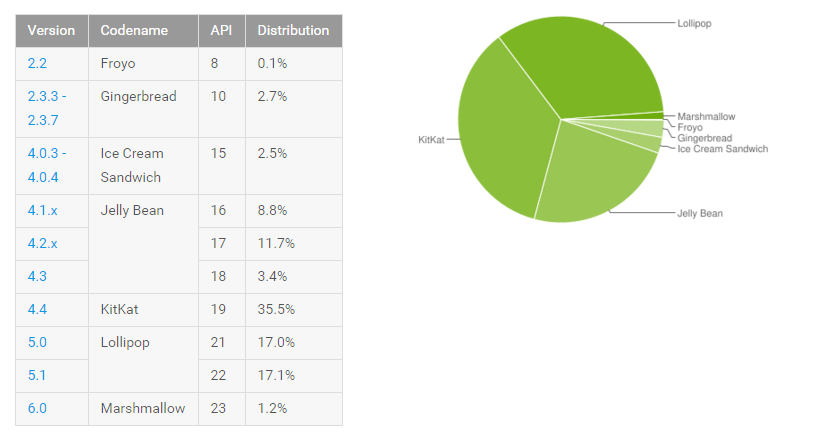
\includegraphics[width=1\textwidth]{figures/android_versionen.png}
	\captionof{figure}{Android Plattform Versionen \cite{platform:versions}}
	\label{figure:androidVersionen}
	\vspace{2ex}
\end{minipage}
 
Die Beispielimplementierung ist ab einer Version größer 5.0 kompatibel. Denn für das Anzeigen der Daten wird eine Funktionalität benötigt, die erst in der API Version 21 enthalten ist. Die App kann dadurch auf mehr als einem Drittel der vertriebenen Geräte ausgeführt werden. Wenn Geräte Systemupdates erhalten, bald auf mehr.

	
	

%%%%%%%%%%%%%%%%%%%%%%%%%%%%%%%%%%%%%%%%%%%%%%%%%%%%%%%%%%%%%%%%%%%%%%%%
\chapter{Rest}
\label{sec:rest}
%%%%%%%%%%%%%%%%%%%%%%%%%%%%%%%%%%%%%%%%%%%%%%%%%%%%%%%%%%%%%%%%%%%%%%%%
Der Architekturstil \acrlong{REST}, kurz \acrshort{REST} wurde erstmals im Jahr 2000 in der Dissertation von Roy Fielding vorgestellt. REST beschreibt dabei ein Konzept, dass die Prinzipien des World Wide Web zusammenfasst. Roy Fielding abstrahierte sich dabei von konkreten Architekturen wie dem \acrfull{HTTP} oder \acrfull{URI}. Er legte nur Kernprinzipien fest, die mit unterschiedlichen Protokollen umgesetzt werden können. Zum Beispiel wie Ressourcen im WEB identifiziert oder adressiert werden \cite{fielding:restDis}. \\
\\
Es werden dabei folgende 5 Kernprinzipien unterschieden \cite{restHttp:book}: 
\begin{enumerate}
	\item \textbf{Ressourcen mit eindeutiger Identifikation}\\
	Durch einen global definierten Namensraum wird sichergestellt, dass Ressourcen weltweit eindeutig identifiziert werden. Im Web heißt dieses Konzept für die Vergabe von IDs, \textit{Uniform Resource Identifier} oder kurz URI. 
	
	\item \textbf{Hypermedia}\\
	Mithilfe dieses Konzeptes ist es mögliche andere Ressourcen zu referenzieren, um beispielsweise an zusätzliche Informationen zu gelangen. Ein weiterer wichtiger Aspekt ist die Möglichkeit die Applikation durch Links zu steuern. Ein Server kann dem Client über Hypermedia-Elemente mitteilen, welche Aktion er als Nächstes auszuführen hat - indem der Client einen Link \textit{folgt}. Dies wird auch oft als das \acrfull{HATEOAS}-Konzept bezeichnet. 
	
	\item \textbf{Standardmethoden}\\
	Jede Ressource unterstützt den gleichen Satz an Methoden, mit dem diese verarbeitet werden können. Bei HTTP zählen dazu folgende:
	\begin{itemize}
		\item GET, für die Dartstellung von Ressourcen
		\item POST, für das Erstellen einer Ressource
		\item PUT, für das Aktualisieren einer Ressource
		\item DELETE, für das Löschen einer Ressource
		\item HEAD, um Methadaten einer Ressource Abzurufen
		\item OPTION, um die unterstützten Methoden einer Ressource zu erhalten
	\end{itemize}
	
	\item \textbf{Unterschiedliche Repräsentationen}\\
	HTTP verfolgte einen Ansatz zur Trennung der Verantwortlichkeiten, für Daten und Operationen. Ein Client der ein bestimmtes Dateiformat verarbeiten kann, ist in der Lage jede Ressource mit diesem Format zu verarbeiten, da die Operationen dafür dieselben sind. 
	
	\item \textbf{Statuslose Kommunikation}\\
	Serverseitig wir der Zustand des Clients nicht gespeichert. Der aktuelle Zustand muss vollständig auf Seiten des Clients abgespeichert werden und bei Reqeuests müssen die nötigen Informationen an den Server übermittelt werden.
	
\end{enumerate}


%%%%%%%%%%%%%%%%%%%%%%%%%%%%%%%%%%%%%%%%%%%%%%%%%%%%%%%%%%%%%%%%%%%%%%%%
\chapter{Vorstellung der Frameworks}
\label{chapter:frameworks}
%%%%%%%%%%%%%%%%%%%%%%%%%%%%%%%%%%%%%%%%%%%%%%%%%%%%%%%%%%%%%%%%%%%%%%%%

In diesem Kapitel werden die einzelnen Frameworks vorgestellt. Zuerst wird ein kurzer allgemeiner Überblick gegeben, bevor genauer auf die Funktionsweise der Frameworks eingegangen wird.
\\\\
Um die Frameworks beschreiben und vergleichen zu können, wurde mit jedem Framework eine eigene App entwickelt. Diese Apps unterscheiden sich dabei nur in der Form der REST Kommunikation, welche auf Basis des jeweiligen Frameworks umgesetzt wurde. Als Build-Tool kommt dabei Gradle zum Einsatz. Gradle ist ein auf Java basierendes Tool, zur Build-Automatisierung und zum Build-Management. Es dient daher der Automatsierng von Builds, Tests und Deployments. Gradle nutzt für einen einfachen Build hauptsächlich die \texttt{build.gradle} Datei, in welcher alle Tasks und Abhängigkeiten eines Projekts definiert sind.

%=======================================================================
\section{Retrofit}
%=======================================================================

\subsection{Allgemein}
Retrofit ist ein typsicherer HTTP Client für Android und Java, welcher von Square Open Source entwickelt wurde und aktuell in der Version 2.0 ausgeliefert wird \cite{retrofit}. Das Framework baut auf OkHttp auf, welches die Kommunikation auf der Netzwerkebene übernimmt \cite{okhttp}. Retrofit sagt über sich selbst:

\begin{center}
	\textit{\textquotedblleft Retrofit turns your HTTP API into a Java interface.\textquotedblright}, \cite[Webseite von Retrofit]{retrofit} 
	\\
\end{center}

Mithilfe von Annotation bei den Interface Methoden wird angegeben wie Request zu verarbeiten sind. Daher muss jede Interface-Methode eine HTTP Annotation besitzen, die angibt welche Request Methode zu verwenden ist \cite{retrofit}. Es stehen dabei fünf built-in HTTP Methoden zur Auswahl GET, POST, PUT, DELETE und HEAD.
\\\\
Standardmäßig kann Retrofit nur \texttt{ResponseBody} und \texttt{RequestBody} von OkHttp serialisieren und deserialisieren. Durch das hinzufügen von Konvertern ist es jedoch möglich, weitere Formate wie \acrfull{JSON} oder \acrfull{XML} zum Übertragen von Daten zu verwenden. Seit der Veröffentlichung von Retrofit in der Version 2, werden auch noch zusätzliche Parser zur Serialisierung und Deserialisierung von JSON-Daten unterstützt. In der Vergangenheit wurde nur die GSON Bibliothek unterstützt, welche daher die am häufigsten verwendete Bibliothek zum Parsen von JSON-Daten darstellt \cite{consumingRetrofit}. Im Rahmen der Bachelorarbeit wird aber die Jackson Bibliothek zum Übertragen von Daten verwendet, da diese am schnellsten Daten serialisiert und deserialisiert  \cite{json:evaluation}.

Die Serverschnittstellen werden durch spezielle Annotationen bei den Interface Methoden spezifiziert, die Details über Parameter und die verwendete Request Methode beinhalten. Es stehen unter anderem folgende Annotationen zur Verfügung:
\newpage
\begin{list}{-}{}
	\item \texttt{@GET}, \texttt{@POST}, \texttt{@PUT}, \texttt{@DELETE}\\
	Diese Annotationen geben an, welche Request Methode zu verwenden ist.
	\item \texttt{@Path} \\
	Durch diese Annotation ist es möglich, die URL des Endpoints dynamisch zu konfigurieren. Dabei wird ein bestimmter Teil in der URL, der durch Klammern gekennzeichnet wurde, durch den dazugehörenden Parameter ersetzt (siehe Listing \ref{retrofitPowerPlantService}, Zeile \ref{line:path}).
	\item \texttt{@Body} \\
	Jeder Parameter der über diese Annotation verfügt, wird in den Body der Request Anfrage eingefügt - nachdem das dazugehörende Java Objekt serialisiert wurde (Listing \ref{retrofitPowerPlantService}, Zeile \ref{line:body}).
\end{list}

\subsection{Funktionsweise}
Um Retrofit verwenden zu können, müssen die Abhängigkeiten aus dem Listing \ref{dependenciesRetrofit} in die \texttt{build. gradle} Datei des Projektes eingefügt werden.

\begin{lstlisting}[language=java, label=dependenciesRetrofit, caption={Retrofit build.gradle}, frame=single]
dependencies {
	compile 'com.squareup.retrofit:retrofit:2.0.0-beta2'
	compile 'com.squareup.retrofit:converter-jackson:2.0.0-beta2'
	compile 'com.squareup.okhttp:okhttp:2.4.0'
	compile 'com.fasterxml.jackson.core:jackson-core:2.6.0'
	compile 'com.fasterxml.jackson.core:jackson-annotations:2.6.0'
}
\end{lstlisting}

Um Requests zur Server Schnittstelle versenden zu können, muss die Retrofit Builder Klasse verwendet werden, welche auch die Basis URL der Server REST-Schnittstelle spezifiziert (siehe Listing \ref{retrofitBuilder}).

\begin{lstlisting}[language=java, caption={Retrofit Builder},label={retrofitBuilder}, frame=single, escapechar=|, stringstyle=\color{mymauve}\scriptsize]
private static final String URL = "https://revex.inso.tuwien.ac.at/api/";
 
public static <S> S createService(Class<S> serviceClass) {

	Retrofit retrofit = new Retrofit.Builder()
			.baseUrl(URL)
			.addConverterFactory(GsonConverterFactory.create())
			.build();
	
	return retrofit.create(serviceClass);
}
\end{lstlisting}

Ist ein return Wert bei einem Request vorhanden, ist dies immer ein parametrisiertes \texttt{Call<T>} Objekt, beispielsweise \texttt{Call <PowerPlant>} (siehe Listing \ref{retrofitPowerPlantService}). Wird kein typenspezifischer Response benötigt oder erwartet, kann als return Wert  \texttt{Call<Response>} angegeben werden. 
\newpage
\begin{lstlisting}[language=java, caption={Auszug aus dem PowerPlantService},label={retrofitPowerPlantService}, escapechar=|, frame=single]
public interface PowerPlantService {

	@GET("powerplants")
	public Call<List<PowerPlant>> getPowerPlants();
	
	@POST("powerplants")
	public Call<PowerPlant> createPowerPlant(@Body PowerPlant powerPlant);
	
	@DELETE("powerplants/{id}")
	public Call<PowerPlant> deletePowerPlantById(@Path("id") int id); |\label{line:path}|
	
	@PUT("powerplants/{id}")
	public Call<PowerPlant> updatePowerPlant(@Path("id") int id, @Body PowerPlant powerPlant); |\label{line:body}|
}
\end{lstlisting}

Sollen bei einem Request noch zusätzlich Daten in den Header eingefügt oder dieser manipuliert werden, ist dies durch das Interface \texttt{Interceptor} möglich (siehe Listing \ref{addToken}). Dadurch kann zum Beispiel vor jeder Anfrage an den Server, ein Token hinzugefügt werden, welches vom Server zur Authentifizierung verwendet wird.

\begin{lstlisting}[language=java, caption={Hinzufügen des Tokens, für gültigen Login},label={addToken}, escapechar=|, frame=single]
public static <S> S createServiceWithAuthToken(Class<S> serviceClass, final AuthToken token) {
	Interceptor interceptor = new Interceptor() {
		@Override
		public Response intercept(Chain chain) throws IOException {
			Request newRequest = chain.request().newBuilder()
				.addHeader("Accept", "application/json")
				.addHeader("X-Auth-Token", token.getToken())
				.build();
		
			return chain.proceed(newRequest);
		}
	};
		
	OkHttpClient client = new OkHttpClient();
	client.interceptors().add(interceptor);
		
	Retrofit retrofit = new Retrofit.Builder()
		.client(client)
		.baseUrl(BASE_URL)
		.addConverterFactory(GsonConverterFactory.create())
		.build();
	
	return retrofit.create(serviceClass);
}
\end{lstlisting}

\newpage
%=======================================================================
\section{Spring for Android}
%=======================================================================

\subsection{Allgemein}
Spring gliedert sich in zahlreiche Projekte, mit dem Ziel die Java Entwicklung zu vereinfachen. Die Idee zum Spring Framework hatte Rod Johnson im Jahr 2003. An den zahlreichen Open Source Projekten von Spring  beteiligen sich weltweit eine große Anzahl von Entwicklern \cite{springITWissen}. Spring for Android ist ein Projekt von Spring, dass die Entwicklung von Andorid-Apps vereinfachen soll. Aktuell wird das Projekt in der Version 2.0 ausgeliefert. Es stellt dabei ausgewählte Komponenten von Spring, gebündelt für Android, zur Verfügung \cite{springForAndroid:website}. Dies sind im speziellen 

\begin{itemize}
	\item ein Rest Client (RestTemplate) und
	\item Authentifikations Unterstützung für Security APIs (OAuth).
\end{itemize}

Spring for Android unterstützt dabei keine Dependency Injection, eine der Kernfunktionen des Core Spring Frameworks. Die Bibliothek unterstützt den Entwickler daher nicht, bei der Umsetzung einer möglichst losen Kopplung in seiner Applikation \cite{springForAndroid:dahanne}.
\\\\
Grundbaustein des Frameworks ist die Klasse \texttt{RestTemplate}, welche Teil des im Jahr 2009 erschienen Framework \textquotedblleft Spring for MVC\textquotedblright\, ist. Diese Klasse ermöglicht Java-Entwicklern eine High-Level-Abstraktion von untergeordneten Java-APIs, wie des HTTP Clients. Die Klasse \texttt{Rest- Template} unterstützt dabei auch die gzip Komprimierung und die Übertragung von JSON und XML Daten, indem \acrfull{POJO} Objekte  – einfache Java-Objekte, die keine Business Logik enthalten \cite{fowler:POJO} – automatisiert konvertiert werden \cite{springForAndroid:dahanne}.
\\\\
Die Klasse \texttt{RestTemplate} ist für den clientseitigen Zugriff auf einen RESTful Service zuständig. Das Verhalten kann durch Callback Methoden und durch konfigurieren des \texttt{HttpMessage- Converter} angepasst werden. Der \texttt{HttpMessageConverter} wird dabei verwendet um einen HTTP Request Body zu erstellen oder den Response in Java Objekte zu konvertieren. Die Klasse \texttt{MappingJackson2HttpMessageConverter} ist dabei ein Message Converter mit dem JSON Daten verarbeitet werden können.

Die Klasse \texttt{RestTemplate} stellt verschiedene Methoden zur Verfügung, um alle gängigen HTTP Methoden verwenden zu können, wie GET, POST, PUT, DELETE, HEAD und OPTION \cite{springDokuRestTemplate}.

\subsection{Funktionsweise}
Um Spring for Android verwenden zu können, muss die Abhängigkeiten aus dem Listing \ref{dependenciesSpring} in die \texttt{build.gradle} Datei des Projektes eingefügt werden.

\begin{lstlisting}[language=java, frame=single, label=dependenciesSpring,  caption={Spring for Android build.gradle}, stringstyle=\color{mymauve}\scriptsize]
dependencies {
	compile 'org.springframework.android:spring-android-rest-template:2.0.0.M1'
	compile 'com.fasterxml.jackson.core:jackson-core:2.6.0'
	compile 'com.fasterxml.jackson.core:jackson-annotations:2.6.0'
}
\end{lstlisting}
\newpage
Wie bereits beschrieben, wird die Klasse \texttt{RestTemplate} dazu verwendet um HTTP Anfragen zusammenzubauen, um mit der Server REST-Schnittstelle kommunizieren zu können. Im Listing \ref{lst:getAllPowerPlants} folgt ein kurzes Beispiel eines GET Requests, um vom Server alle vorhanden Kraftwerke zu erhalten.

\begin{lstlisting}[language=java, caption={GET Request um alle Kraftwerke zu erhalten},label=lst:getAllPowerPlants, frame=single, tabsize=3]
public static List<PowerPlant> getPowerPlants() {
  RestTemplate restTemplate = new RestTemplate(
			new BufferingClientHttpRequestFactory(
				new SimpleClientHttpRequestFactory()));
				  
  restTemplate.getMessageConverters().
	  add(new MappingJackson2HttpMessageConverter());
 
 URI url = UriComponentsBuilder.
		 fromUriString(ServiceGenerator.BASE_URL).
		 path("/powerplants").build().toUri();
 
 HttpHeaders headers = new HttpHeaders();
 headers.set("X-Auth-Token", 
	 UtilitiesManager.getInstance().getAuthToken().getToken());

 headers.setContentType(MediaType.APPLICATION_JSON);
 
 HttpEntity entity = new HttpEntity(headers);
 
 HttpEntity<PowerPlant[]> response = restTemplate.
		 exchange(url, HttpMethod.GET, entity, PowerPlant[].class);
 
 return Arrays.asList(response.getBody());
}
\end{lstlisting}

Wie man anhand des Beispieles sehen kann, erfolgt eine automatisierte Umwandlung der erhaltenen JSON Daten zu einem Java Objekt. Für einen GET Request muss daher nur der Endpunkt des Servers und der Typ der Response Daten spezifiziert werden. Um HTTP-Header Felder hinzuzufügen wird ein \texttt{HttpHeaders} Objekt benötigt, diesem können dann die HTTP Felder über die \texttt{set}-Methode hinzugefügt werden. Dadurch ist es möglich vor jeder Anfrage das X-Auth-Token hinzuzufügen, welches vom Server für die Authentifizierung verwendet wird.
\\\\
Um die Daten zu einem speziellen Kraftwerk abzufragen, ist es nötig die URL dynamisch zur Laufzeit zu verändern. Dabei wird das abzufragende Kraftwerk über den Parameter \texttt{id} (siehe Listing \ref{lst:springGet}, Zeile 3) spezifiziert.

\begin{lstlisting}[language=java, caption={Abfrage der Daten zu einem speziellen Kraftwerke},label={lst:springGet}, frame=single]
URI url = UriComponentsBuilder.
		fromUriString(ServiceGenerator.BASE_URL).
		path("/powerplants/" + id).
		build().toUri();
		
HttpEntity entity = new HttpEntity(headers);

HttpEntity<PowerPlant> response = restTemplate.
		exchange(url, HttpMethod.GET, entity, PowerPlant.class);		
		
\end{lstlisting}

\newpage
Ein POST Request mit Spring for Android kann aus dem Listing \ref{postSpring} entnommen werden.

\begin{lstlisting}[language=java, caption={POST Request um ein neues Kraftwerke anzulegen}, label=postSpring, frame=single, tabsize=3]
HttpHeaders headers = new HttpHeaders();

headers.set("X-Auth-Token", 
		 UtilitiesManager.getInstance().getAuthToken().getToken());
		 
headers.setContentType(MediaType.APPLICATION_JSON);
 
HttpEntity<PowerPlant> requestEntity = 
		 new HttpEntity<>(powerPlant,headers);
 
HttpEntity<PowerPlant> response = restTemplate.
	exchange(url, HttpMethod.POST, requestEntity, PowerPlant.class);
\end{lstlisting}

Im Objekt \texttt{requestEntity} sind dabei die Daten enthalten, die im Body des HTTP Requests übertragen werden.

\newpage
%=======================================================================
\section{Jersey}
%=======================================================================

\subsection{Allgemein}
In Java gibt es mit JAX-RS einen Standard zum Implementieren von REST-basierten Webservices. Dieser wurde in der JSR-311 "JAX-RS: The Java API for RESTful Web Services" \cite{jsr311} genauer spezifiziert und ist deshalb ein offizieller Teil von Java. Das Jersey Framework ist dabei eine robuste Open-Source Referenz Implementierung der Spezifikation \cite{restfulWS:Kubert}.
\\\\
Die JAX-RS-Client-API Implementierung von Jersey kann mit einem beliebigen Web-Service, der auf das HTTP-Protokoll aufsetzt, kommunizieren. Der Jersey-Client wird zurzeit in der Version 2.22.1 ausgeliefert. Der serverseitige Endpoint muss nicht unbedingt mit JAX-RS implementiert sein, jedoch muss der HTTP Standard eingehalten werden.
\\\\
Den Grundbaustein der Jersey-Client Implementierung bildet die Klasse \texttt{ClientBuilder}. Diese wird dazu verwendet neue \texttt{Client}-Instanzen anzulegen, über welche Requests zum Server versendet werden. Mithilfe der \texttt{ClientBuilder}-Klasse können auch zusätzliche Eigenschaften für den \texttt{Client} definiert werden, wie zum Beispiel die SSL Transport Konfiguration. Des weiteren kann ein \texttt{Client} mithilfe der \texttt{ClientConfig}-Klasse speziell konfiguriert werden, diese Konfiguration wird bei der Erstellung des \texttt{Client} einer Factory Methode übergeben. Mithilfe der \texttt{ClientConfig}-Klasse können Provider registriert oder Filter hinzugefügt werden. Ein oft verwendeter Filter ist zum Beispiel der \texttt{LoggingFilter}. Dieser ist ein Protokollierungsfilter, der die Kommunikation zwischen Server und Client aufzeichnet und dessen Aufzeichnung später für Debugging Zwecke genutzt werden kann \cite{jersey:doku}. 
\\\\
Nachdem eine \texttt{Client}-Instanz erfolgreich erstellt wurde, kann mit dieser Instanz ein \texttt{WebTarget} Objekt erzeugt werden, welches den Endpoint zum Server spezifiziert. Um nun erfolgreich einen HTTP Request abzusetzen, muss ein \texttt{Invocation.Builder} Objekt erzeugt werden. Dieses Objekt wird dazu genutzt um die Anfrage zum Server genauer zu konfigurieren und abzusenden. Es gibt sowohl Methoden um den Media Type des Request und Response anzugeben, die HTTP Methode zu definieren und den HTTP Header genauer zu spezifizieren \cite{jersey:doku}.
\\\\
Die Client API von Jersey unterstützt alle gängigen HTTP Methoden, welche GET, POST, PUT, DELETE, HEAD und OPTION sind \cite{invocation:api}.

\subsection{Verwendung unter Android}
\label{workaroundAndroid}
Jersey kann erst ab der Version 2.16 auf Android verwendet werden. Davor war es nicht möglich Jersey auf Android auszuführen, aufgrund der Abhängigkeit des Client Core Moduls zum package \texttt{javax.xml.stream}, welches in der Android Java API nicht vorkommt. In der neuen Jersey Version wurden alle JAXB-B Provider Abhängigkeiten in ein eigenes Modul ausgelagert \cite{jerseyAndroid:podlesak}. Fügt man nun die Abhängigkeit zu diesem Modul in das Projekt ein, funktioniert die grundlegende Kommunikation zwischen einem Android Jersey Client und den REST Server. 

\begin{lstlisting}[language=java,numbers=none]
compile 'javax.xml.bind:jaxb-api:2.1'
\end{lstlisting}
 
Dennoch ist es noch immer nicht möglich, den Jersey Client ohne Abhängigkeitsproblemen in einer Android Umgebung zu verwenden. Es werden noch immer Abhängigkeiten zu packages benötigt, die in der Android-Umgebung nicht verfügbar sind. Mithilfe der HK2 API ist es möglich Komponenten ohne Vorbereitung aus dem HK2 Service Locator zu entfernen. Der Workaround aus dem Listing \ref{lst:workaround} hilft Fehler durch fehlende Abhängigkeiten zu unterdrücken und dennoch alle Funktionen des Jersey Clients in der Android Umgebung zu unterstützen \cite{jerseyAndroid2:podlesak}.

\begin{lstlisting}[language=java, caption={Workaround Jersey Client auf Android},label={lst:workaround}, escapechar=|, frame=single]
public static class AndroidFriendlyFeature implements Feature {
	
	@Override
	public boolean configure(FeatureContext context) {
		context.register(new AbstractBinder() {
		
			@Override
			protected void configure() {
				addUnbindFilter(new Filter() {
				
					@Override
					public boolean matches(Descriptor d) {
					  String implClass = d.getImplementation();
					  return implClass.startsWith(
						"org.glassfish.jersey.message.internal.DataSource")
						|| implClass.startsWith(
					   "org.glassfish.jersey.message.internal.RenderedImage");
					}
				});
			}
		});
		return true;
	}
}
\end{lstlisting}

Das Feature für den Workaround muss später noch bei der \texttt{Client}-Instanz registriert werden.

\begin{lstlisting}[language=java, , numbers=none, frame=single]
client = ClientBuilder.newClient().
							register(AndroidFriendlyFeature.class);
\end{lstlisting}


\subsection{Funktionsweise}
Hat man alle erforderlichen Abhängigkeiten zum Projekt hinzugefügt, kann ein einfacher GET Request realisiert werden, der ein \texttt{PowerPlant} Objekt zurückgibt (siehe Listing \ref{lst:jerseyGET}). Der Media Type wird mithilfe der \texttt{accept}-Methode spezifiziert, die Art der HTTP Request Methode wird durch \texttt{get(PowerPlant.class)} angegeben. Dabei wird durch den Parameter in der Methode der Returntyp des Response festgelegt, in diesem Fall wird genau ein Objekt des Typs \texttt{PowerPlant} erwartet. 

\begin{lstlisting}[language=java, caption={GET Request},label={lst:jerseyGET}, escapechar=|, frame=single]
public static PowerPlant getPowerPlantById(int id) {
	
	ClientConfig clientConfig = new ClientConfig().
					register(JacksonFeature.class);
	
	Client client = ClientBuilder.newClient(clientConfig).
					register(AndroidFriendlyFeature.class);
	
	Invocation.Builder builder = client.
					target(BASE_URL).
					path("/powerplants/" + id).
					request(MediaType.APPLICATION_JSON);
	
	PowerPlant powerPlant = builder.
					accept(MediaType.APPLICATION_JSON).
					get(PowerPlant.class);
	
	return powerPlant;
}
\end{lstlisting}

Im Listing \ref{lst:jerseyPOST} wird ein POST Request abgesendet, der ein Objekt an den Server im JSON Format übergibt und auch einen Returnwert im JSON Format erwartet. 
\begin{lstlisting}[language=java, label={lst:jerseyPOST}, escapechar=|,numbers=none, frame=single]
PowerPlant newPowerPlant = builder.
			accept(MediaType.APPLICATION_JSON).
			post(Entity.entity(powerPlant, MediaType.APPLICATION_JSON), 
					PowerPlant.class);

\end{lstlisting}

\newpage
%=======================================================================
\section{AndroidAnnotations}
%=======================================================================
\label{androidannoations}
\subsection{Allgemein}
AndroidAnnotations ist ein Projekt das von Pierre-Yves Ricau gestartet wurde. Der Kern des Projektteams besteht aus aktiven und ehemaligen eBusinessInformation Mitarbeitern. Das Unternehmen unterstützt das Open Source Projekt durch seine Mitarbeiter, indem diesen Zeit und Ressourcen zur Verfügung gestellt werden, um an AndroidAnnotations zu arbeiten. Das Projekt wird aktuell in der Version 4.0 ausgeliefert \cite{annotation:sponsors}. 
\\\\
Das Projekt AndroidAnnotations soll dabei helfen, Codefragemente die sich bei der Android-App Entwicklung wiederholen, zu reduzieren, indem Annotationen verwendet werden. Dadurch verringert sich der zu schreibende und wartende Code, wodurch die Entwicklung beschleunigt und die Wartbarkeit verbessert werden kann \cite{annotation:introduction}. 
\\\\
Bei der Kompilierung des Codes werden die verwendeten Annotationen aufgelöst, wodurch es zu keiner Laufzeitbeeinträchtigung durch die Verwendung von AndroidAnnotations kommt. Dies geschieht indem eine Unterklasse jeder einzelnen Aktivität erzeugt wird und die Annotations durch die zugrundeliegenden Codefragmente ersetzt werden. Wird beispielsweise eine \texttt{MyActivity} Klasse implementiert, erzeugt AndroidAnnotations die entsprechende \texttt{MyActivity\_} Unterklasse. Ein kleiner Nachteil dieses Ansatzes ist, dass ein Unterstrich hinter den Namen der einzelnen Aktivitäten in der Manifest-Datei anhängt werden muss. Des weiteren muss beim Starten einer neuen Aktivität auch darauf geachtet werden, dass die entsprechend generierte Unterklasse verwendet wird \cite{annotation:spring}. 
\\\\
Die Rest API von AndroidAnnotations ist dabei ein Wrapper rund um das Spring for Android \texttt{RestTemplate} Modul. Die \texttt{@Rest}-Annotation über einem Interface ist dabei der Grundbaustein, welche die Schnittstelle genauer spezifiziert. Die Endpoint URL vom Server wird über den \texttt{rootUrl} Parameter bei der \texttt{@Rest}-Annotation angegeben. Des weiteren muss bei der \texttt{@Rest}-Annotation mindestens ein Messagekonverter angegeben werden, welcher dem Spring \texttt{Http- MessageConverters} entspricht, da dieser dem RestTemplate Modul zur Verfügung gestellt wird. Dadurch werden automatisiert Java Objekte serialisiert und deserialisiert. Sind mehrere Konverter definiert, durchläuft Spring alle, bis der Content-Typ des Requests oder Response verarbeitet werden kann. Es können auch Interceptoren hinzugefügt werden, welche beispielsweise jeden Request protokollieren oder benutzerdefinierte Authentifizierung handhaben \cite{annotation:rest}.
\\\\
Wichtige Annotationen für die Rest Kommunikation sind \cite{annotation:rest}:
 
\begin{itemize}
	\item \texttt{@Get}, \texttt{@Post}, \texttt{@Put},\texttt{@Delete}, \texttt{@Head}, \texttt{@Options}\\
	Über diese Annotationen wird die Request Methode spezifiziert, die Rest API von AndroidAnnotations unterstützt dabei die selben HTTP Methoden wie Spring for Android.
	\item \texttt{@Path}\\
	Methodenparameter die mit dieser Annotation versehen werden, sind ausdrücklich als Pfadvariablen markiert, sie müssen daher einen entsprechenden Platzhalter in der URL haben.
	\item \texttt{@Body}\\
	Diese Annotation wird dazu verwendet, um Daten in den Body eines Requests einzufügen. Diese Annotation kann nur in Kombination mit den HTTP-Methoden POST, PUT, DELETE oder PATCH verwendet werden. Außerdem is nur ein \texttt{@Body} Parameter pro Request zulässig.
\end{itemize}

\subsection{Funktionsweise}

Um AndroidAnnotations verwenden zu können, müssen die Abhängigkeiten aus dem Listing \ref{dependenciesAndroidAnnoations} in die \texttt{build.gradle} Datei eingefügt werden.

\begin{lstlisting}[language=java,label=dependenciesAA,stringstyle=\color{mymauve}\scriptsize, label=dependenciesAndroidAnnoations,  caption={AndroidAnnotations build.gradle}, frame=single]
apply plugin: 'com.android.application'
apply plugin: 'com.neenbedankt.android-apt'

dependencies {
	apt "org.androidannotations:androidannotations:4.0-SNAPSHOT"
	compile "org.androidannotations:androidannotations-api:4.0-SNAPSHOT"
	compile "org.androidannotations:rest-spring:4.0-SNAPSHOT"
	compile 'org.springframework.android:spring-android-rest-template:1.0.1.RELEASE'
	compile 'com.fasterxml.jackson.core:jackson-core:2.6.0'
	compile 'com.fasterxml.jackson.core:jackson-databind:2.6.0'
}

apt {
	arguments {
		androidManifestFile variant.outputs[0].processResources.manifestFile
	}
}
\end{lstlisting}

Das Android-apt Plugin hilft bei der Verarbeitung und richtigen Auflösung der Annotationen. Beispielsweise muss AndroidAnnotations wissen, wo die dazugehörige Manifest-Datei liegt. Dies wird durch die  \texttt{variant} angegeben. Durch die Angabe eines Indexes können auch unterschiedliche Manifest-Dateien für verschiedene Anwendungsfälle spezifiziert werden \cite{android:apt}.
\\\\
Die beispielhafte Implementierung eines AndroidAnnotation Rest Client kann man aus folgendem Listing \ref{lst:aaServiceRequests} entnehmen. Durch Annotationen wird sowohl die Serverschnittstelle, also auch die zu verwendenden HTTP Methoden spezifiziert. Zur Konvertierung der übertragenen Daten im JSON Format wird die Klasse \texttt{MappingJackson2HttpMessageConverter} von Jackson API verwendet.

\begin{lstlisting}[language=java, caption={Auszug aus dem PowerPlantService Interface},label={lst:aaServiceRequests}, escapechar=|, frame=single]
@Rest(rootUrl = "https://revex.inso.tuwien.ac.at/api",
		converters = { MappingJackson2HttpMessageConverter.class },
		interceptors = { HttpBasicAuthenticatorInterceptor.class })
public interface PowerPlantService {
	@Get("/powerplants")
	List<PowerPlant> getPowerPlants();
	
	@Post("/powerplants")
	public PowerPlant createPowerPlant(@Body PowerPlant powerPlant);

	@Delete("/powerplants/{id}")
	PowerPlant deletePowerPlantById(@Path int id);

	@Put("/powerplants/{id}")
	PowerPlant updatePowerPlant(@Path int id, @Body PowerPlant pp);
}
\end{lstlisting}

Beim Listing \ref{lst:aaService} wird auch ein Interceptor registriert, der vor jeden Requests das benutzerdefinierte Authentifizierungs-Token in dem Header einfügt.

\begin{lstlisting}[language=java, caption={Interceptor für das setzen eines zusätzlichen HTTP Header Feldes},label={lst:aaService}, escapechar=|, frame=single]
public class HttpBasicAuthenticatorInterceptor  
										implements ClientHttpRequestInterceptor {

	@Override
	public ClientHttpResponse intercept(HttpRequest request, 
			byte[] data, ClientHttpRequestExecution execution) 
			throws IOException {
					
		request.getHeaders().add("X-Auth-Token", 
			UtilitiesManager.getInstance().getAuthToken().getToken());
			
		return execution.execute(request, data);
	}
}
\end{lstlisting}

\subsection{zusätzliche Dienste}
Einer der größten Vorteile dieses Frameworks ist, dass zur Verfügung stellen weiterer Dienste. Ein solcher Dienst  ist die \acrfull{DI}. Durch die Verwendung dieses Entwurfsmusters wird die Kopplung zwischen einzelnen Modulen (Objekte, Klassen) reduziert. Dabei bekommen die Module ihre Abhängigkeiten von einer zentralen Komponente zugewiesen \cite{annotation:spring}. Die anderen getesteten Frameworks beinhalten keine DI-Komponente, können aber mit entsprechenden Bibliotheken um diese Funktionalität erweitert werden. 

Die Haupteigenschaften des Projektes sind unter anderem \cite{annotation:introduction}:

\begin{itemize}
	\item \textbf{Dependency Injection}\\
	Injection von Views, System Services oder Ressourcen.
	\item \textbf{einfaches Threading-Modell}\\
	Annotation über Methoden, die angeben, ob die Methode vom UI-Thread oder von einem Hintergrundthread ausgeführt werden soll.
	\item \textbf{Event Binding}\\
	Annotation über Methoden um Events von Views zu behandeln, es werden keine anonymen Listener Klassen mehr benötigt.
	\item \textbf{Rest Client}\\
	Durch erstellen eines Client Interfaces, wird die zugrundeliegende Implementierung generiert.
\end{itemize}
%%%%%%%%%%%%%%%%%%%%%%%%%%%%%%%%%%%%%%%%%%%%%%%%%%%%%%%%%%%%%%%%%%%%%%%%
\chapter{Vergleich}
\label{sec:comparison}
%%%%%%%%%%%%%%%%%%%%%%%%%%%%%%%%%%%%%%%%%%%%%%%%%%%%%%%%%%%%%%%%%%%%%%%%
Es folgt nun eine Gegenüberstellung der einzelnen Frameworks, anhand der in Kapitel \ref{sec:methodik} definierten Kriterien. Als erster wird ein genereller Überblick über die einzelnen Fakten zu den Frameworks gegeben und deren Unterschiede beschrieben. Danach wird genauer auf relevanten Kriterien für das Revex Projekt eingegangen und ein persönliches Fazit zu den Frameworks gegeben.

\section{Gegenüberstellung der Frameworks}

{\large \textbf{Entwicklungskultur rund um die Frameworks}}\\\\
Alle Frameworks werden unter einer Open Source Lizenz zur Verfügung gestellt. Einige Lizenzen beinhalten aber ein Copyleft, was verlangt, dass die entwickelte Software ebenfalls wieder unter der gleichen Lizenz als \acrfull{OSS} zur Verfügung gestellt wird. Die wichtigste Copyleft-Lizenz ist die \acrfull{GPL}. Die GPL bestimmt, dass Software, welche eine Framework unter dieser Lizenz nutzt, wiederum nur unter GPL vertrieben werden darf. Die Apache License ist eine Lizenz ohne Copyleft, es ist daher zulässig Frameworks mit dieser Lizenz in proprietärer Software zu verwenden. Die \acrfull{CDDL} beinhaltet ein abgeschwächtes Copyleft, lizenzierter Code kann in einem anderen Framework verwendet werden, solange dieser Code nicht auf Dateiebene gemischt wird. Die CDDL verbietet nicht, entwickelte Software unter einer anderen Lizenz zu veröffentlichen. Für die reinen Nutzer von OSS, welche die Frameworks weder weiterentwickeln noch vertreiben wollen, spielen die Unterschiede der verschiedenen OSS-Lizenzen kaum eine Rolle. Will ein Entwickler jedoch seine Arbeitsergebnisse nicht als OSS veröffentlichen, darf er für seine Arbeiten keine OSS Frameworks verwenden, welche mit einem strengen Copyleft lizenziert sind \cite{openSource}. Die Lizenzen der einzelnen Frameworks könnten aus der Tabelle \ref{tableVergleich} entnommen werden.
\\\\
OSS wird durch Communities entwickelt, weiterentwickelt und gewartet. Dabei übernimmt die Community zahlreiche Aufgaben, die bei Closed Software vom Hersteller oder Anbieter wahrgenommen werden. In der Regel gibt es zu jeder OSS genau eine Community. User der Software können dabei registriertes Mitglied der Community sein und aktiv am Projekt als Entwickler oder Tester mitarbeiten. Die Qualität einer Software hängt dabei maßgeblich von der Aktivität und der Struktur der Community ab. Sind zahlreiche aktive Mitglieder mit unterschiedlichen Rollen am Projekt beteiligt, ist dies eine Grundlage für eine gute Qualität der Software \cite{openSource:community}. Alle untersuchten Frameworks weisen eine aktive und starke Community auf.
\\\\
Um die Anwendung neuer Frameworks zu lernen, lesen 78 Prozent der Entwickler die Dokumentation, 55 Prozent verwenden Codebeispiele und 29 Prozent fragen Kollegen \cite{robillard:apis}. Dadurch ist es besonders wichtig auf eine aktuelle Dokumentation des Source-Codes Zugriff zu haben. Wird nur eine veraltete Dokumentation zur Verfügung gestellt, kann es passieren das die entwickelte Software Sicherheitslücken hat oder mehr Zeit für eine korrekte Implementierung benötigt wird \cite{lethbridge:documentation}. Für alle Frameworks ist eine Dokumentation vorhanden. Die Dokumentation von Retrofit deckt dabei aber nur die grundlegend Funktionsweise ab und ist im Vergleich zu den anderen schwächer. Ein Problem hierbei ist, dass gerade ein großes Update des Frameworks durchgeführt wurde und die vorhandene Dokumentation dadurch teilweise veraltet ist. Es konnten auch Codebeispiele für alle Frameworks gefunden werden, diese sind gut erklärt und ermöglichen es eine lauffähige Anwendung zu implementieren. Problematisch war es allerdings die gefunden Jersey Codebeispiele unter Android zu starten, da keines dieser speziell für Android entwickelt wurde. Es musste zuerst ein Workaround (siehe Kapitel \ref{workaroundAndroid}) durchgeführt werden, um die Beispiele auf einem Android Gerät starten zu können.
\\\\
{\large \textbf{Implementierung der REST-Frameworks}}\\\\
Einer der relevantesten Aspekte für den Evaluierungsprozess ist die Implementierung und Verwendungsweise der Frameworks. Bis auf Jersey sind alle Frameworks leicht einzubinden und zu benützen. Für Jersey muss zuerst ein Workaround durchgeführt werden, damit dieses Framework überhaupt unter Android genutzt werden kann. Die genaue Verwendungsweise der Frameworks wird in Kapitel \ref{chapter:frameworks} beschrieben.
\\\\
Es werden von allen Frameworks die gängigsten HTTP-Methoden unterstützt. Retrofit unterstützt dabei als einziges nicht die HTTP-Methode OPTIONS. Es ist auch möglich mit allen Frameworks den HTTP-Header zu erweitern bzw. zu verändern. Des weiteren ist es auch möglich alle möglichen Medientypen zu unterstützten, wenn ein Konverter dafür implementiert und beim Framework registriert wird. Endpoint URLs zum Server können dynamisch während der Laufzeit bei allen Frameworks verändert werden. 
\\\\
Wenn zeitraubende Aktionen ausgeführt werden sollen, wie z.B. das Herunterladen einer großen Dateien aus dem Internet, langweilen sich User oft. Denn diese müssen dann warten bis der Request vollständig abgearbeitet wurde und können währenddessen nicht weiterarbeiten. Dies kann aber verhindert werden, indem zeitraubende Aktion im Hintergrund ausgeführt werden - in Form von asynchronen Requests \cite{louis:android}. Mithilfe aller Frameworks können asynchrone Requests modelliert werden. 
\\\\
Das HATEOAS Konzept wird von Jersey und Spring for Android unterstützt. Jedoch muss bei Spring for Android eine eigene Bibliothek \textquotedblleft Spring HATEOAS\textquotedblright eingebunden werden, damit eine Linkverfolgung möglich ist. Wenn das HATEOAS Konzept mit AndroidAnnotations verwendet werden soll, muss ebenfalls \textquotedblleft Spring HATEOAS\textquotedblright eingebunden werden und die Verwendung ist nur ohne Annotations möglich. Man greift dabei auf die Basis REST Implementierung zurück, welche Spring for Android ist. Retrofit unterstützt das HATEOAS Konzept nicht.
\\\\
Das registrieren von Error Handlern ist bei allen Frameworks möglich, dadurch können aussagekräftige Fehlermeldungen für den User erzeugt werden. Designrichtlinien für mögliche Geräte geben an, dass es sinnvoll ist Rückmeldungen für Aktion des Systems zu geben, wie beispielsweise eine Fehlermeldung, wenn der Server nicht erreichbar ist. Eine solche Rückmeldung sollte für den Benutzer verständlich sein. Zum Beispiel sind die Fehlermeldungen \textquotedblleft HTTP404 ERROR\textquotedblright und \textquotedblleft Diese Seite konnte nicht gefunden werden \textquotedblright äquivalent, die zweite Fehlermeldung ist aber für einen größteil der User verständlicher \cite{gong2004guidelines}.
\\\\
{\large \textbf{Performance}}\\\\
Mobile Geräte haben längst Einzug in das Alltagsleben erhalten, viele Nutzer erweitern die Funktionalität der Geräte mit zahlreichen Anwendungen. Jede installierte App auf einen mobilen Endgerät hat Einfluss auf den Energieverbrauch. Je mehr Anwendungen auf eine Endgerät installiert sind und je öfter diese genutzt werden, desto höher ist der Energieverbrauch und die Betriebszeit sinkt dadurch massiv \cite{Wil2012}. Daher ist bei der Entwicklung darauf zu achten, das der Energieverbrauch so gering wie möglich gehalten wird. Auswirkungen auf den Energieverbrauch eines Smartphones haben sowohl der Bildschirm, die \acrfull{CPU}, die Kommunikation über das Mobilfunknetz, als auch das WLAN-Modul. Werden die einzelnen Komponenten so wenig wie möglich beansprucht, ist der Energieverbrauch der Anwendung gering \cite{vetter}. 
\\\\
Umso länger und mehr Daten bei einem Request über das Mobilfunknetz oder das WLAN-Modul übertragen werden, desto mehr Energie wird verbraucht. Es sollte daher darauf geachtet werden, dass die Requestdauer möglichst gering ist und nicht unnötige Daten übertragen werden. Des weiteren ist die Rechenleistung von Smartphones  wesentlich geringer als jene von Notebooks, um die Betriebszeit zu erhöhen. Daher ist bei der Entwicklung auch darauf zu achten, dass die CPU Beanspruchung der Apps gering gehalten wird, damit das System performant weiterarbeiten kann \cite{mittal:energy}. Außerdem sollte die benötigte CPU Leistung aus einem weiteren Grund möglichst gering sein, den die Hardware variiert von Smartphone zu Smartphone. Ist die benötigte CPU Leistung gering, ist es möglich die App auf nahezu allen mobilen Geräten zu installieren und zu starten \cite{joorabchi:challenges}. 
\\\\
Für den Performance Vergleich wurden daher sowohl die CPU-Auslastung, als auch die Dauer für GET- und POST Requests (Dauer der Netzwerkkommunikation) der einzelnen Frameworks gegenübergestellt. Um Vergleichswerte zu ermitteln, wurden jede App einzeln in einem Emulator gestartet und die gleich Abfolge an Funktionsaufrufen durchgeführt. 
\\\\
Die Zeitdauer der GET-Requests bei der Abbildung \ref{getRequests} setzt sich aus 11 einzeln abgesetzte GET-Requests zusammen. Diese Requests werden benötigt, um die Details zu einem bestimmten Kraftwerke anzuzeigen. Es werden in der Praxis oft mehrere GET-Request hintereinander abgesetzt, daher wurde die Dauer ermittelt um alle Details zu einem Kraftwerk abzurufen. Es konnte dabei festgestellt werden, dass Retrofit die Daten am schnellsten überträgt, dicht gefolgt von AndroidAnnotations und Jersey am langsamsten ist.

\begin{figure} [ht]
	\centering
	\subfloat[GET Request Retrofit]{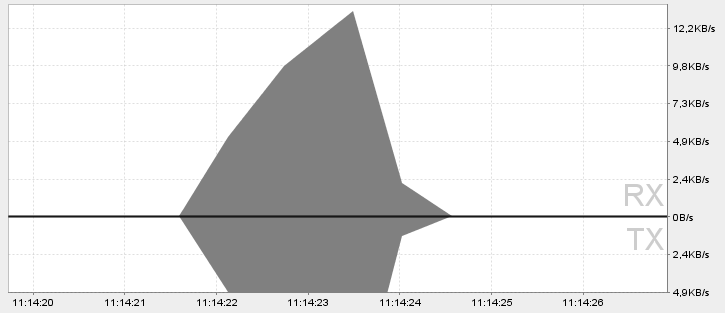
\includegraphics[width=0.45\textwidth]{figures/get_retrofit.png}} \qquad
	\subfloat[GET Request Jersey]{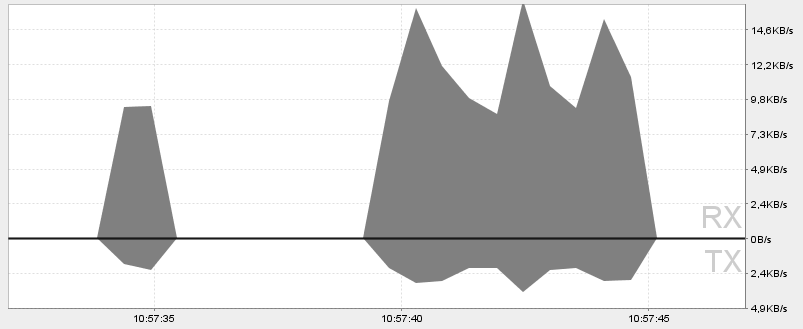
\includegraphics[width=0.45\textwidth]{figures/get_jersey.png}} \qquad
	\subfloat[GET Request Spring for Android]{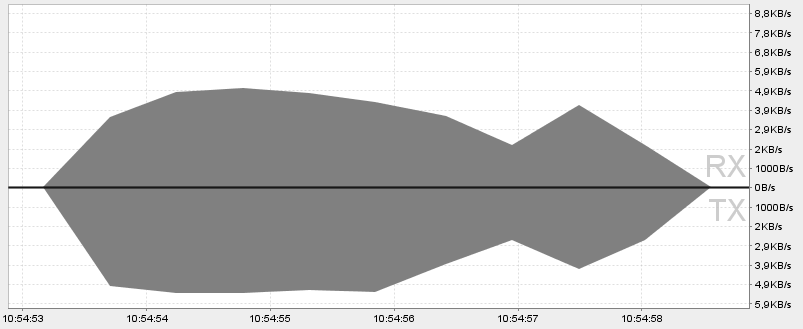
\includegraphics[width=0.45\textwidth]{figures/get_spring.png}} \qquad
	\subfloat[GET Request AndroidAnnotations]{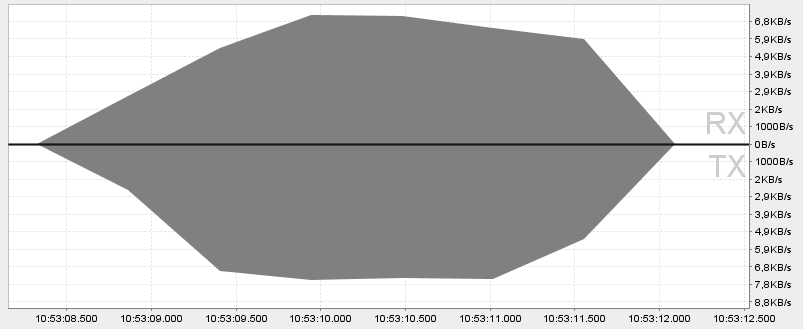
\includegraphics[width=0.45\textwidth]{figures/get_aa.png}}
	\caption{Zeitmessung der GET Requests} 
	\label{getRequests}
\end{figure} 

\newpage
Die Messung der Zeitdauer für einen POST Request ist aus der Abbildung \ref{postRequests} zu entnehmen. Dabei wurde die Zeit gemessen bis neu eingegeben Daten, um ein Kraftwerk anzulegen erfolgreich zum Server übermittelt wurden. Es konnte dabei festgestellt werden, dass alle Frameworks circa gleich lange benötigen, um die Daten zu übertragen. Spring for Android ist dabei minimal langsamer als die anderen, dies ist aber zu vernachlässigen, da diese Verzögerung keine Auswirkung auf die Usability für einen User hat \cite{meyer:performance}.

\begin{figure} [ht]
	\centering
	\subfloat[POST Request Retrofit]{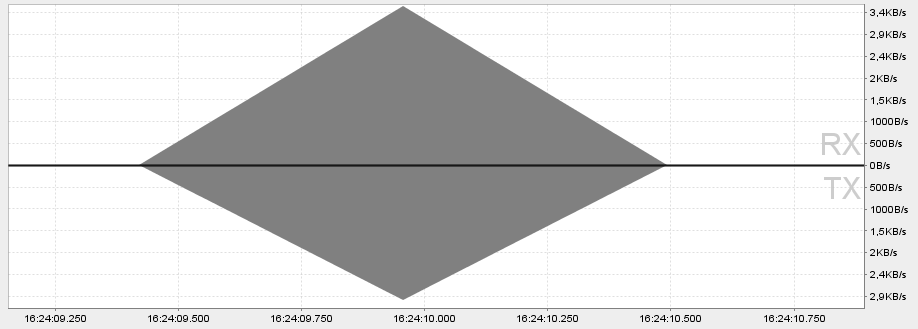
\includegraphics[width=0.45\textwidth]{figures/post_retrofit.png}} \qquad
	\subfloat[POST Request Jersey]{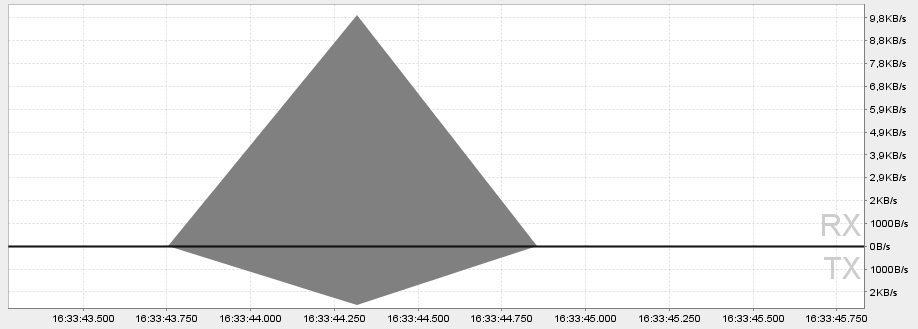
\includegraphics[width=0.45\textwidth]{figures/post_jersey.png}} \qquad
	\subfloat[POST Request Spring for Android]{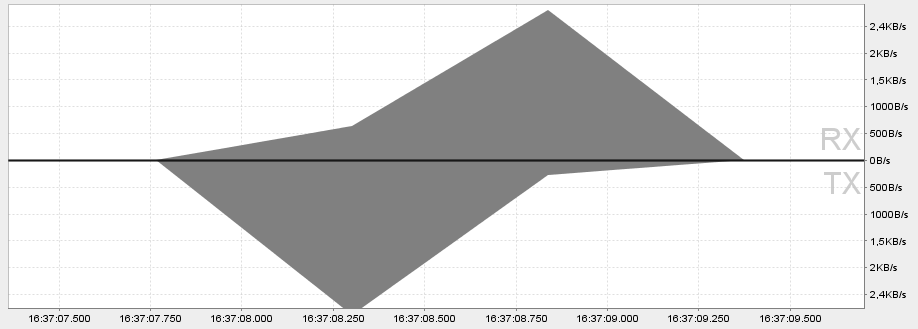
\includegraphics[width=0.45\textwidth]{figures/post_spring.png}} \qquad
	\subfloat[POST Request AndroidAnnotations]{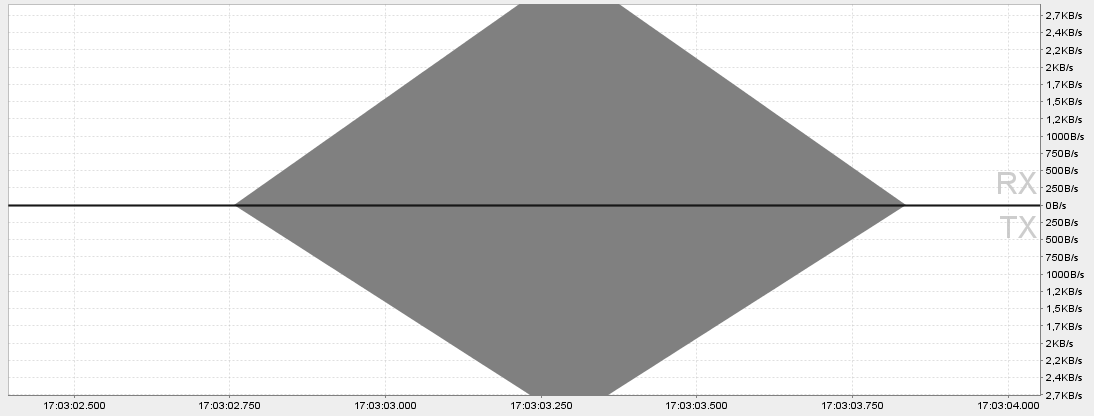
\includegraphics[width=0.45\textwidth]{figures/post_aa.png}}
	\caption{Zeitmessung der POST Requests} 
	\label{postRequests}
\end{figure} 

In der Abbildung \ref{cpuAuslastung} wird die CPU Auslastung der einzelnen Frameworks gegenübergestellt. Aus dieses Abbildung kann entnommen werden, das AndroidAnnotations die CPU am geringsten in Anspruch nimmt und Jersey am stärksten. Bei der Benutzung der Apps ist auch festzustellen, dass AndroidAnnotations und Retrofit am schnellsten arbeiten und eine flüssige Bedienung der Anwendung möglich ist. Jersey ist des öfteren langsam und hat kleine Ruckler währende der Bedienung.  

\begin{figure} [ht]
	\centering
	\subfloat[CPU Auslastung Retrofit]{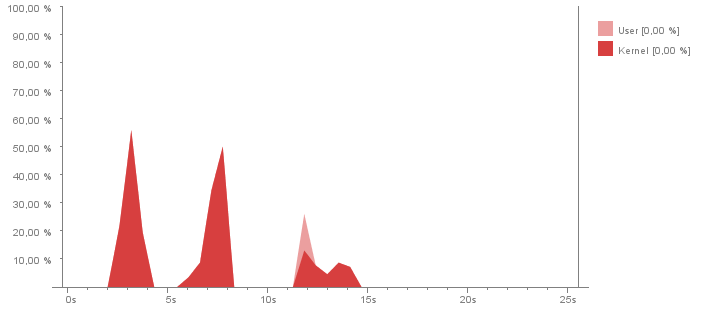
\includegraphics[width=0.45\textwidth]{figures/cpu_retrofit.png}} \qquad
	\subfloat[CPU Auslastung Jersey]{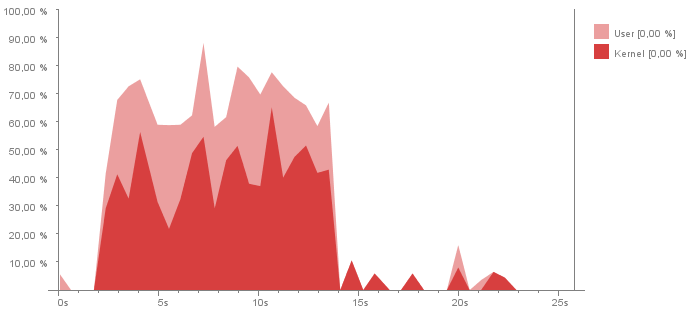
\includegraphics[width=0.45\textwidth]{figures/cpu_jersey.png}} \qquad
	\subfloat[CPU Auslastung Spring for Android]{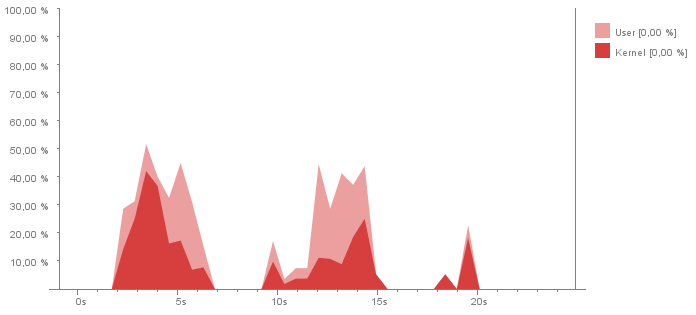
\includegraphics[width=0.45\textwidth]{figures/cpu_spring.png}} \qquad
	\subfloat[CPU Auslastung Request AndroidAnnotations]{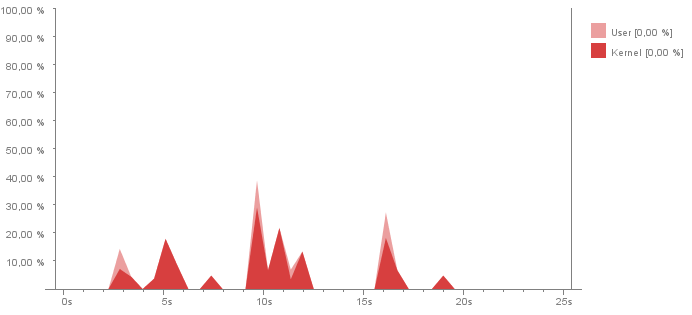
\includegraphics[width=0.45\textwidth]{figures/cpu_aa.png}}
	\caption{CPU Auslastung} 
	\label{cpuAuslastung}
\end{figure} 

{\large \textbf{Speicherplatz}}\\\\
Eine der größten Herausforderungen beim Implementieren von Apps ist der Hardwareunterschied der mobilen Geräte. Die Hardwarekomponenten unterscheiden sich nicht nur in der Displaygröße oder CPU Leistung, sondern auch im Speicherbereich \cite{joorabchi:challenges}. Sei es nun der zur Verfügung gestellte \acrfull{RAM} oder interne Speicher, welcher gelegentlich durch Speicherkarten erweitert werden kann. Je mehr und je größere Apps installiert werden, desto mehr leidet die Performance – insbesondere auf älteren oder Hardware schwachen Geräten. Auch spielt die Installationszeit eine wichtige Rolle. User wollen Apps so schnell wie möglich nutzen, längere Installationszeiten sorgen schneller dafür, dass die Installation abgebrochen wird \cite{schaefers:apk}. Bei der Gegenüberstellung der APK Größe und der maximalen RAM Beanspruchung schnitt AndroidAnnotations am besten ab, Jersey am schlechtesten (siehe Tabelle \ref{tableVergleich}). 

\begin{figure} [ht]
	\centering
	\subfloat[benötigter RAM Retrofit]{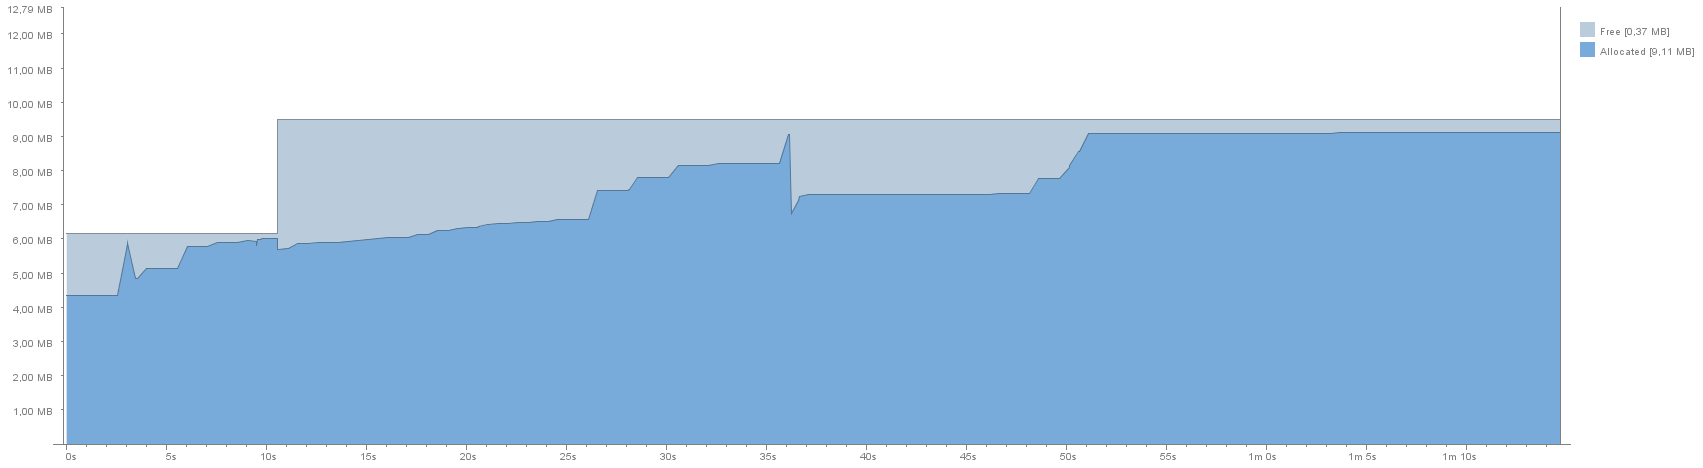
\includegraphics[width=0.48\textwidth]{figures/ram_retrofit.png}} \qquad
	\subfloat[benötigter RAM Jersey]{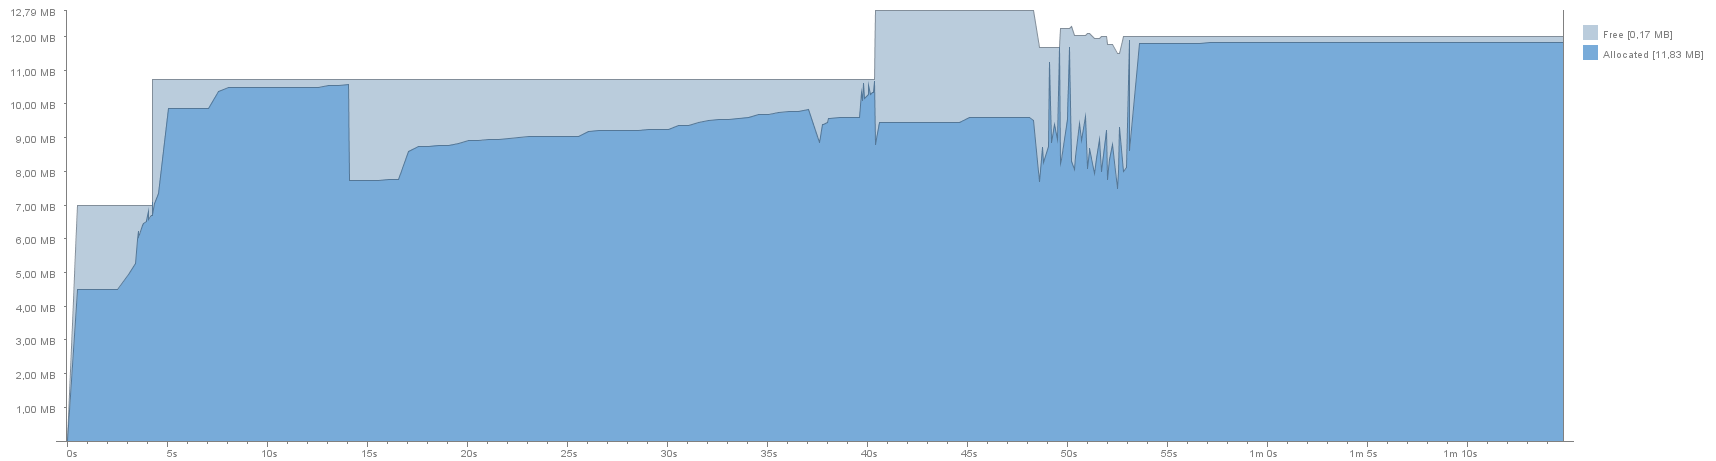
\includegraphics[width=0.45\textwidth]{figures/ram_jersey.png}} \qquad
	\subfloat[benötigter RAM Spring for Android]{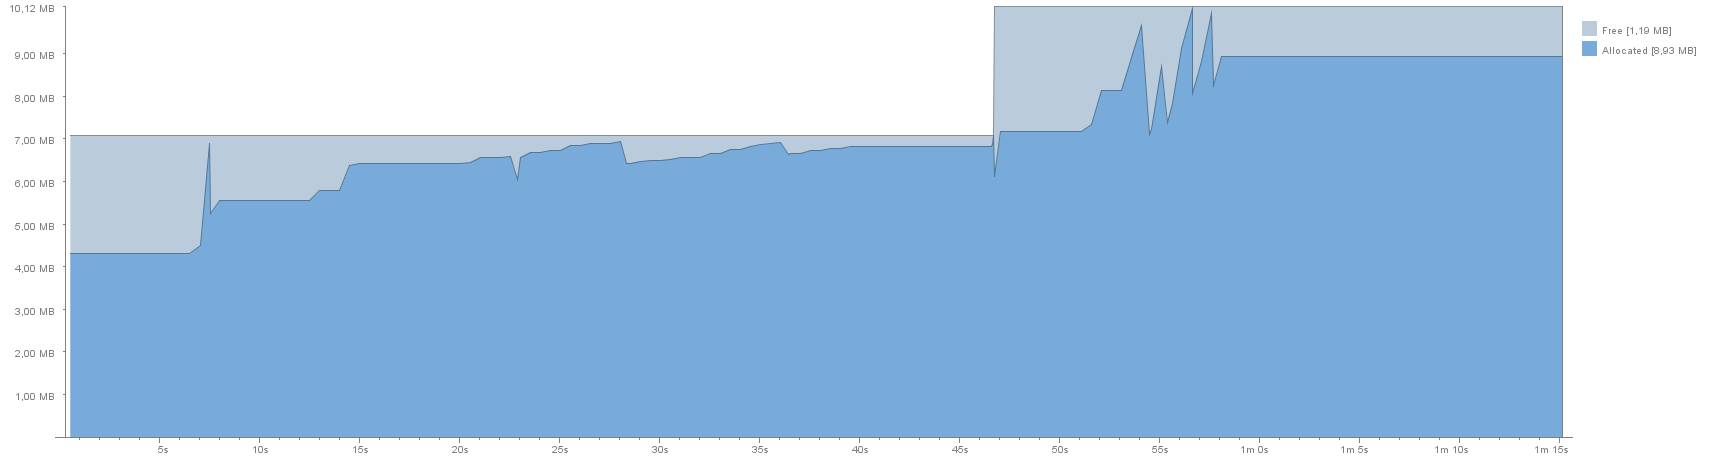
\includegraphics[width=0.45\textwidth]{figures/ram_spring.png}} \qquad
	\subfloat[benötigter RAM Request AndroidAnnotations]{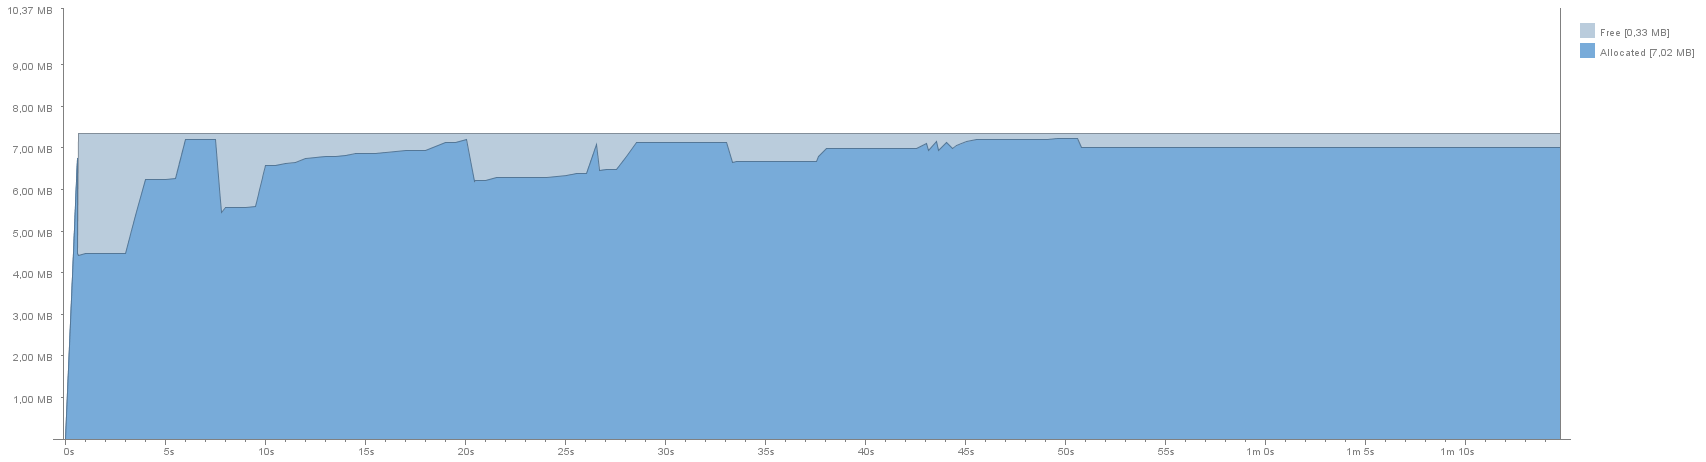
\includegraphics[width=0.45\textwidth]{figures/ram_aa.png}}
	\caption{benötigter RAM} 
	\label{ramB}
\end{figure} 

{\large \textbf{Erweiterte Technische Fähigkeiten der Frameworks}}\\\\
Sicherheit ist ein wesentliches Thema in der Informatik und auch für mobile Geräte. Denn die Apps sind nicht nur auf Informationen des Smartphones beschränkt, sondern haben auch Zugriff auf das Internet. OAuth ist ein Webstandard für den beschränkten Zugriff von Benutzer-Ressourcen auf Servern \cite{shehab:secure}. Dieser Standard wir von allen Frameworks unterstützt und ermöglicht einen sicheren und beschränkten Zugriff auf Ressourcen. 
\\\\
Alle evaluierten Frameworks unterstützten keine weiteren Übertragungsprotokolle außer HTTP. Die ACID-Eigenschaften werden auch von keinem der Frameworks implementiert. Soll aber ein Transaktionsmanagement clientseitig unterstützten werden, muss eine eigene Implementierung geschrieben werden. Dabei muss besonders darauf geachtet werden, dass alle Daten, die während einer Transaktion verwendet werden, gesperrt sind und sich nicht ändern dürfen so lange bis die Transaktion Commited wird oder ein Rollback durchgeführt wird \cite{braun:Transaktionen}.
\\\\
Jersey hat eine serverseitige Referenzimplementierung. Für Spring for Android existiert ebenfalls eine Referenzimplementierung aus der Spring Familie. AndroidAnnoations hat keine direkt Referenzimplementierung, aber man kann auch auf jene der Spring Familie zurückgreifen - den die REST Implementierung von AndroidAnnoations basiert auf Spring for Android. Retrofit hat keine serverseitige Referenzimplementierung.
\\\\
AndroidAnnotations stellt als einziges Framework zusätzliche Dienste bereit, welche die Implementierung einer Android App erleichtern. Diese zusätzlichen Dienste sind unter anderem Dependency Injection oder Event Binding, siehe Kapitel \ref{androidannoations}.
  
\begin{landscape}
% m{3.5cm}|m{4.5cm}|m{4.5cm}|m{4.5cm}|m{4.5cm}
\renewcommand{\arraystretch}{1.3}
\begin{longtable}{m{3.5cm}|m{4.5cm}|m{4.5cm}|m{4.5cm}|m{4.5cm}}
	%	>{\centering \arraybackslash}m{3.5cm}|
	%	>{\centering \arraybackslash}m{4.5cm}|
	%	>{\centering \arraybackslash}m{4.5cm}|
	%	>{\centering \arraybackslash}m{4.5cm}|
	%	>{\centering \arraybackslash}m{4.5cm}}

      \caption{Gegenüberstellung der Frameworks} \\
	  \label{tableVergleich}	 
	  
	    & \textbf{Retrofit} & \textbf{Jersey} & \textbf{Spring for Android}  & \textbf{AndroidAnnotations}  \\  \hhline{=====}
	   \multicolumn{5}{c}{\textbf{Entwicklungskultur}} \\ \hhline{=====}
	  \textbf{Lizenz} &
	  Apache License Version 2.0 & CDDL Version 1.1 \newline GPL Version 2 & 
	  Apache License Version 2.0 & 
	  Apache License 2.0 \newline CDDL \\ \hline
	  \textbf{aktive Community} & Ja & Ja & Ja & Ja\\ \hline
	  \textbf{Dokumentation} & grundlegend & gut & gut  & gut \\ \hline 
		  \textbf{Codebeispiele} &  Ja  & nicht speziell für Android & Ja & Ja\\ \hhline{=====}
	  
	  \multicolumn{5}{c}{\textbf{Implementierung}} \\ \hhline{=====}
	  \textbf{Einbindung} & leicht & problematisch & leicht & leicht \\ \hline
	  \textbf{HTTP-Methoden} & GET, POST, PUT, DELETE, HEAD & GET, POST, PUT, DELETE, HEAD, OPTIONS  & GET, POST, PUT, DELETE, HEAD, OPTIONS & GET, POST, PUT, DELETE, HEAD, OPTIONS \\ \hline
	  \textbf{HTTP-Header} & erweiterbar & erweiterbar & erweiterbar & erweiterbar \\ \hline
	  \textbf{unterstützte\newline Medientypen} & alle möglichen, wenn Konverter für Typ vorhanden ist & alle möglichen, wenn Konverter für Typ vorhanden ist & alle möglichen, wenn Konverter für Typ vorhanden ist & alle möglichen, wenn Konverter für Typ vorhanden ist \\ \hline
	  \textbf{URL veränderbar} & Ja & Ja & Ja & Ja  \\ \hline
	  \textbf{asynchrone Requests} & Ja & Ja & Ja & Ja \\ \hline
	  \textbf{HATEOAS Konzept} & Nein & Ja & mithilfe von Spring HATEOAS & ohne Annotations und mithilfe von Spring HATEOAS \\ \hline 
	  \textbf{Error-Handling} & unterstützt & unterstützt & unterstützt & unterstützt \\ \hline
	 \newpage \hhline{=====}
	  
	  \multicolumn{5}{c}{\textbf{Performance und Speicherplatz}} \\ \hhline{=====}
	  
	  \textbf{GET Request} & \textasciitilde3s & \textasciitilde12s  & \textasciitilde5s & \textasciitilde3.5s\\ \hline
	  
	  \textbf{POST Request} & \textasciitilde1s &  \textasciitilde1s & \textasciitilde1.5s & \textasciitilde1s \\ \hline
	  
	  \textbf{CPU Auslastung} & max. \textasciitilde55\%  & max. \textasciitilde87\% & max. \textasciitilde52\% & max. \textasciitilde40\%\\ \hline
	  \textbf{belegter RAM} & max. 9.11 MB & max. 11.83 MB & max. 8.93 MB & max 7.02 MB \\ \hline
	  \textbf{APK Größe} & 1.70 MB & 2.58 MB & 1.69 MB & 1.44 MB \\ \hhline{=====}

	   \multicolumn{5}{c}{\textbf{Erweiterte Technische Fähigkeiten}} \\ \hhline{=====}
	   
	   \textbf{Sicherheit} & OAuth2, SSL via OkHttp & OAuth2, SSL & OAuth2, SSL & OAuth2, SSL \\ \hline
	   \textbf{andere Protokolle außer HTTP} &  Nein & Nein & Nein & Nein\\ \hline	   
	   \textbf{ACID-Eigenschaften} & Nein & Nein & Nein & Nein \\ \hline
	   \textbf{Server Implementierung} & Nein & Ja &  Spring Framework & Nein (eventuell Spring Framework) \\ \hline
	   \textbf{zusätzliche Dienste} & Nein & Nein & Nein & Ja \\ \hline
 
\end{longtable}
\end{landscape}

\section{Relevante Aspekte für Revex2020}
Für die Implementierung einer App sind sowohl Retrofit, Spring for Android und AndroidAnnoations geeignet. Von Jersey als REST Framework ist abzuraten, da dieses Framework nur mithilfe eines Workarounds benützt werden kann. Darüber hinaus schneidet Jersey im Performance- und Speichervergleich am schlechtesten ab. Vergleicht man nun jene anderen drei ist der Unterschied minimal. Retrofit weißt eine etwas schwächere Dokumentation auf, da gerade eine neue Version erschienen ist und die Dokumentation teilweise noch nicht an die neueste Version angepasst wurde. Spring for Android ist im Lesezugriff langsamer, was einen minimalen Nachteil darstellt - da dies das Hauptaugenmerk einer Implementierung für Revex ist. Retrofit und AndroidAnnoations haben einen leicht zu lesenden Code, da dieser Annotations basiert ist. Dadurch verringert sich der zu schreibende und wartende Code, wodurch die Entwicklung beschleunigt und die Wartbarkeit verbessert werden kann. Der größte Vorteil von AndroidAnnoations sind die zusätzlicher Dienste, welche die Implementieren einer Android App erleichtern.

\section{Persönliches Fazit zu den Frameworks}
Es folgt nun ein kurzer persönlicher Eindruck zu den Frameworks. Wo sind Probleme während der Implementierung aufgetreten und welche Aspekte besonders positiv aufgefallen sind.
\\\\
\textbf{Jersey}
\\\\
\textbf{Retrofit}
\\\\
\textbf{Spring for Android}
\\\\
\textbf{AndroidAnnotations}
\\\\
%%%%%%%%%%%%%%%%%%%%%%%%%%%%%%%%%%%%%%%%%%%%%%%%%%%%%%%%%%%%%%%%%%%%%%%%
\chapter{Zusammenfassung}
\label{sec:summary}
%%%%%%%%%%%%%%%%%%%%%%%%%%%%%%%%%%%%%%%%%%%%%%%%%%%%%%%%%%%%%%%%%%%%%%%%
Diese Arbeit hat sich mit der Evaluierung von REST Frameworks für Android im Kontext des Revex2020 Projektes auseinandergesetzt. Die ausgewählten Frameworks wurden anhand einer Beispielimplementierung vorgestellt und verglichen.
\\\\
Zu Beginn der Arbeit wurde auf einen der größten Trends am Business-Markt eingegangen. Dieser ist die Mobilisierung der Geschäftswelt, wobei unabhängig von Stakeholdern, Zeit, Ort und Geräten auf Daten und Anwendungen zugriffen werden soll. Ein wesentlicher Innovationsstrang ist dabei die Entwicklung von Business-Apps. Mobile Endgräte werden in bestehende Geschäftsprozesse der Unternehmen integriert und greifen dabei oft auf definierte Schnittstellen oder angebotene Dienste zu  \cite{smartMobileApps1}. Herkömmliche Software rückt dabei immer weiter in den Hintergrund, Daten sind sofort und überall abrufbar. Mobile Endgeräte wie Smartphones und Tablets verändern daher die Geschäftswelt nachhaltig, da Unternehmensinformationen jederzeit verfügbar sind - die Unternehmen der Zukunft sind mobil \cite{smartMobileApps7}.
\\\\
In einem Teil der Arbeit werden die verwendeten Technologien Android und REST beschrieben. Android ist ein Betriebssystems, welches primär für Smartphones und Tablets konzeptioniert ist  \cite{overviewAndroid:singh}. Durch die quelloffene Struktur des Betriebssystems ist Android bei vielen Konsumenten und Entwicklern sehr beliebt, wodurch viele Unternehmen ihre mobilen Applikationen auf dieses Betriebssystem ausrichten \cite{statsticMobileOS}. Aufgrund dessen wurde die Evaluierung der REST Frameworks auch auf Android ausgerichtet. In einer kurze Zusammenfassung wurde auf REST als Architekturstil eingegangenen und die 5 Kernprinzipien dieses Stils beschrieben \cite{restHttp:book}.
\\\\
Mithilfe der prototypisch entwickelten Android-App soll es Mitarbeitern zukünftig möglich sein, den Zustand einzelner Kraftwerkskomponenten vor Ort zu erfassen oder Details zum Kraftwerk anzuzeigen. Die App soll auf das bereits vorhandene Backend, eines REST-Webservices zugreifen und diesen verwenden. Um auf das vorhandene Backend zuzugreifen muss ein REST Framework verwendet werden, dass für Android kompatibel ist und performant arbeitet. Um geeignete Rest Frameworks zu finden, wurde eine Technologierecherche durchgeführt und die drei populärsten und den Anforderungen adäquatesten Frameworks für eine Beispielimplementierung ausgewählt.
\\\\
Die Qualität der einzelnen Frameworks wurde anhand definierter Kriterien evaluiert. Diese Kriterien umfassen sowohl die Entwicklungskultur, den Implementierungsprozess und einen Performance- und Speichervergleich. Die ausgewählten REST Frameworks wurden anhand einer Beispielimplementierung vorgestellt und deren Verwendungsweise beschrieben. Im Anschluss daran wurden die einzelnen Frameworks mittels der definierten Kriterien verglichen. Durch die Evaluierung der Frameworks konnte festgestellt werden, dass AndroidAnnotations am besten für die Implementierung der Revex2020 App geeignet ist. Als Abschluss wurde noch ein kurzes persönliches Resümee zu den Frameworks gezogen.


% insert bibliography and such stuff
\BackMatter
\cleardoublepage

%\appendix
%%%%%%%%%%%%%%%%%%%%%%%%%%%%%%%%%%%%%%%%%%%%%%%%%%%%%%%%%%%%%%%%%%%%%%%%%
\chapter{\appendixlabel}
%%%%%%%%%%%%%%%%%%%%%%%%%%%%%%%%%%%%%%%%%%%%%%%%%%%%%%%%%%%%%%%%%%%%%%%%



\end{document}
